\chapter{The Student IDE}
\label{ch:system}

\section{Architecture}
\begin{figure}[ht]
  \centering
  \tikzfig{pipeline}
  \caption{The Student IDE pipeline. Parts 3--5 are the novel contribution.}
  \label{fig:pipeline}
\end{figure}

\section{Event logging editor}
\todo{What is logged (key down/up, paste, edit, cursor, run, error,
snapshot), timing precision, tech stack and why. Screenshot in
\texttt{snapshots/}. Feeds from brain entries tagged 04-system-design.}

\subsection{Student interface}
The student-facing screens (sign-in, consent, task picker, editor, run
output) were redesigned once the logger worked
(\cref{fig:ui-before-after}). The interface is React with Tailwind CSS
and the Motion animation library, on top of a small shared design system
(colour tokens with light and dark themes, motion presets and UI
primitives) that the teacher timeline will reuse.

Motion is deliberately kept away from timing capture. The CodeMirror
editor is created once and never re-rendered, so a keystroke causes no
interface work beyond CodeMirror's own; animations run only on discrete
actions (a run finishing, the finish dialog) and touch only opacity and
transform so the browser can composite them off the main thread; and key
times are taken from the browser event timestamp, not from when a handler
runs. The end-to-end test confirms the event stream is unchanged
(214 events of the same types before and after) and asserts that no main
thread task longer than \SI{50}{\milli\second} overlaps the typing window.
The consent text is unchanged; the motion respects the operating system's
reduced-motion setting.

\begin{figure}[ht]
  \centering
  \begin{subfigure}{0.48\textwidth}
    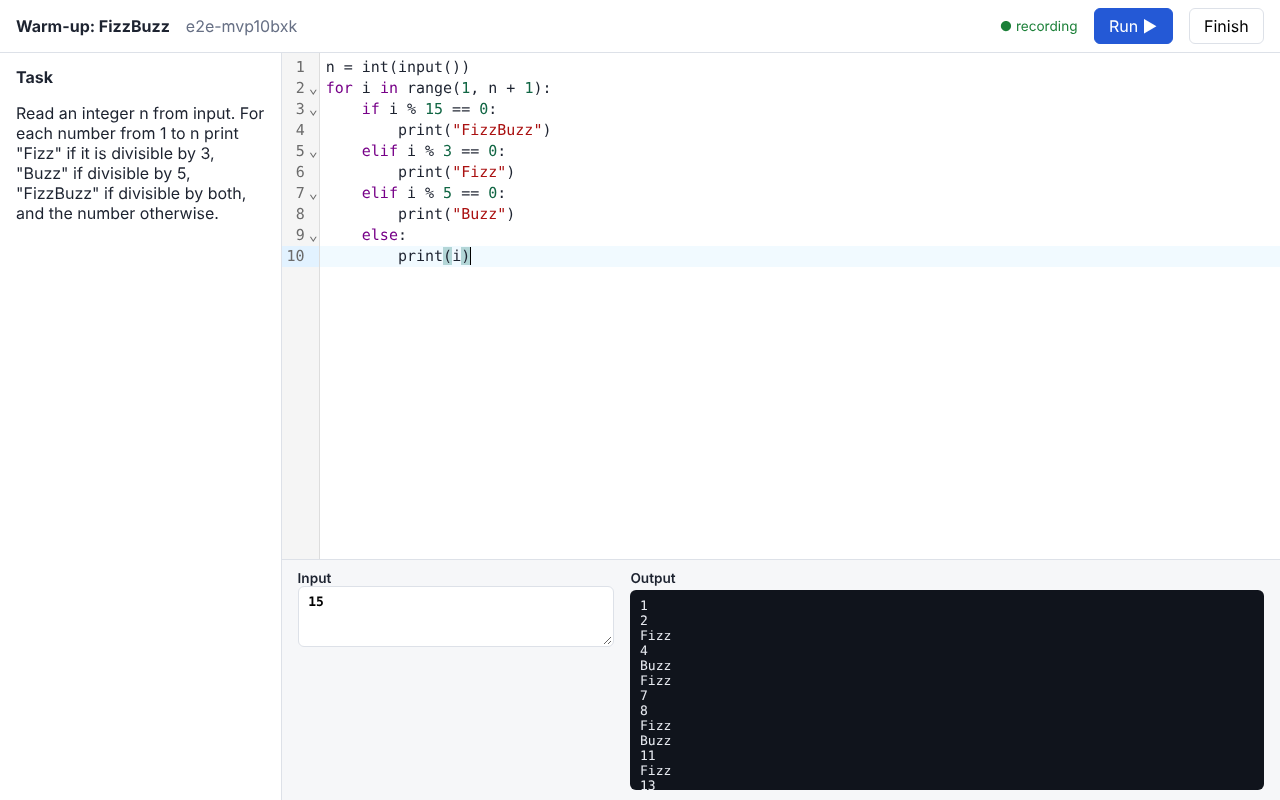
\includegraphics[width=\linewidth]{ui-redesign/before-04-editor}
    \caption{Phase 1 editor}
  \end{subfigure}\hfill
  \begin{subfigure}{0.48\textwidth}
    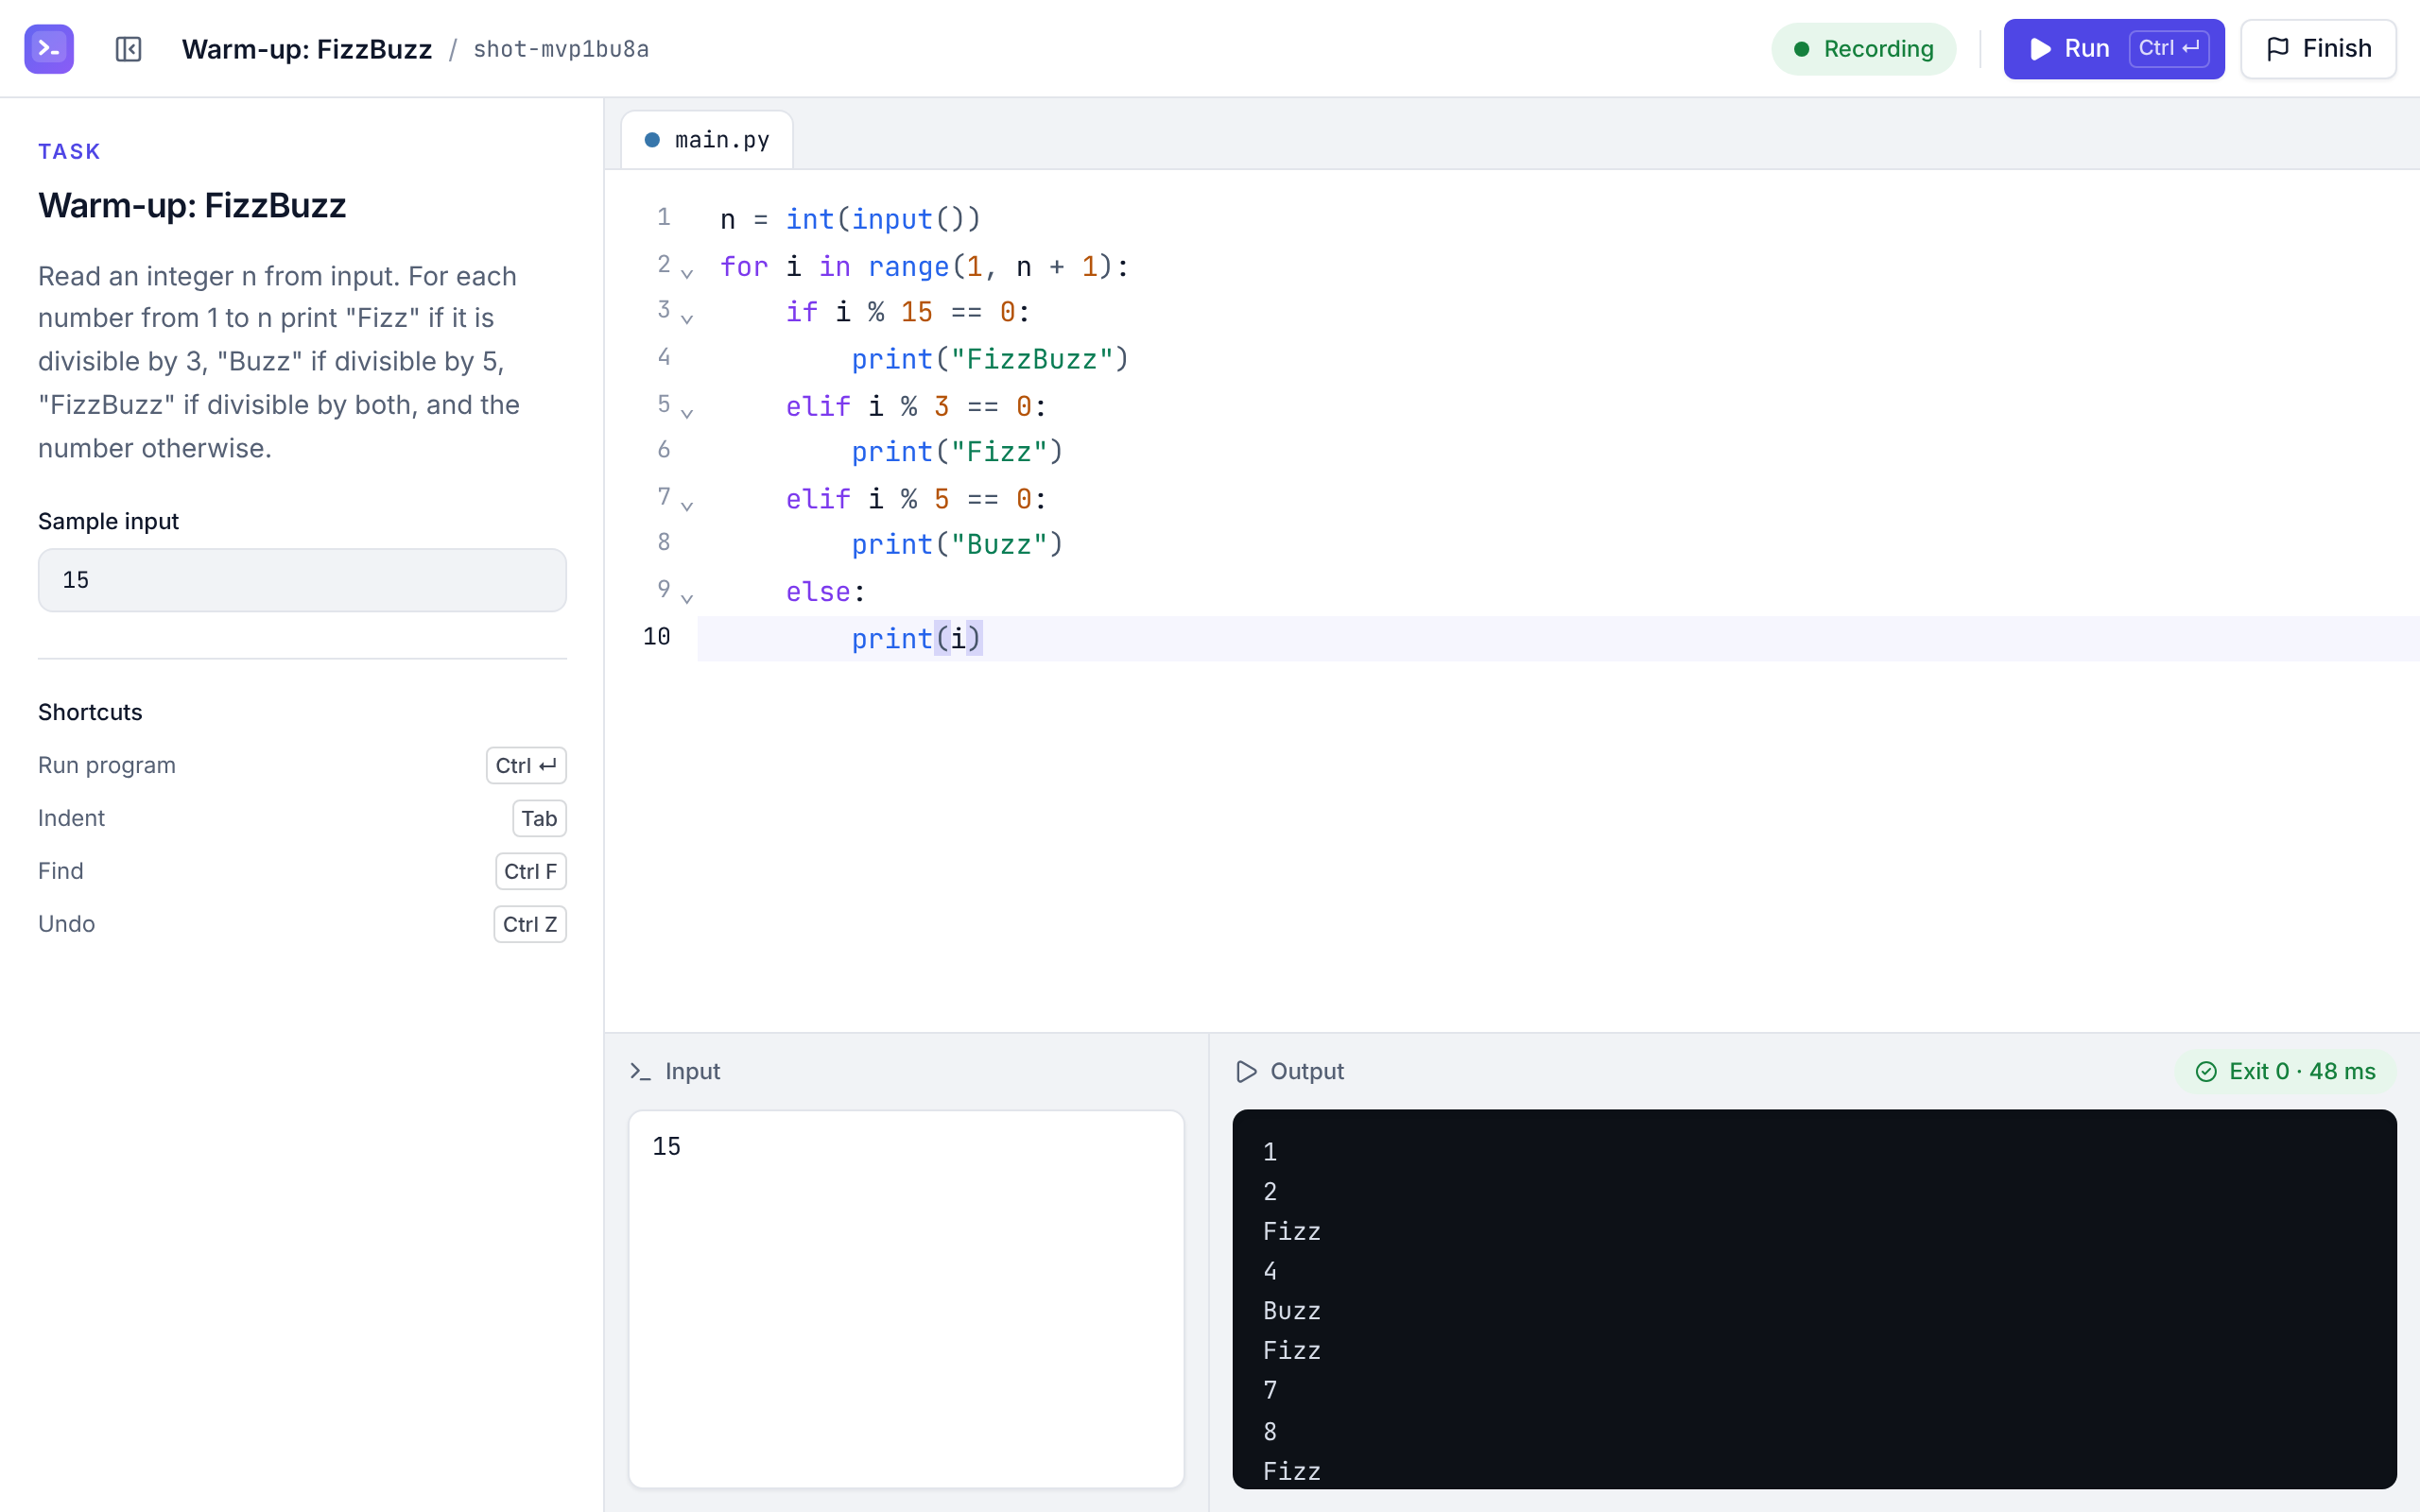
\includegraphics[width=\linewidth]{ui-redesign/after-light-05-run-output}
    \caption{Redesigned editor after a run}
  \end{subfigure}\\[1ex]
  \begin{subfigure}{0.48\textwidth}
    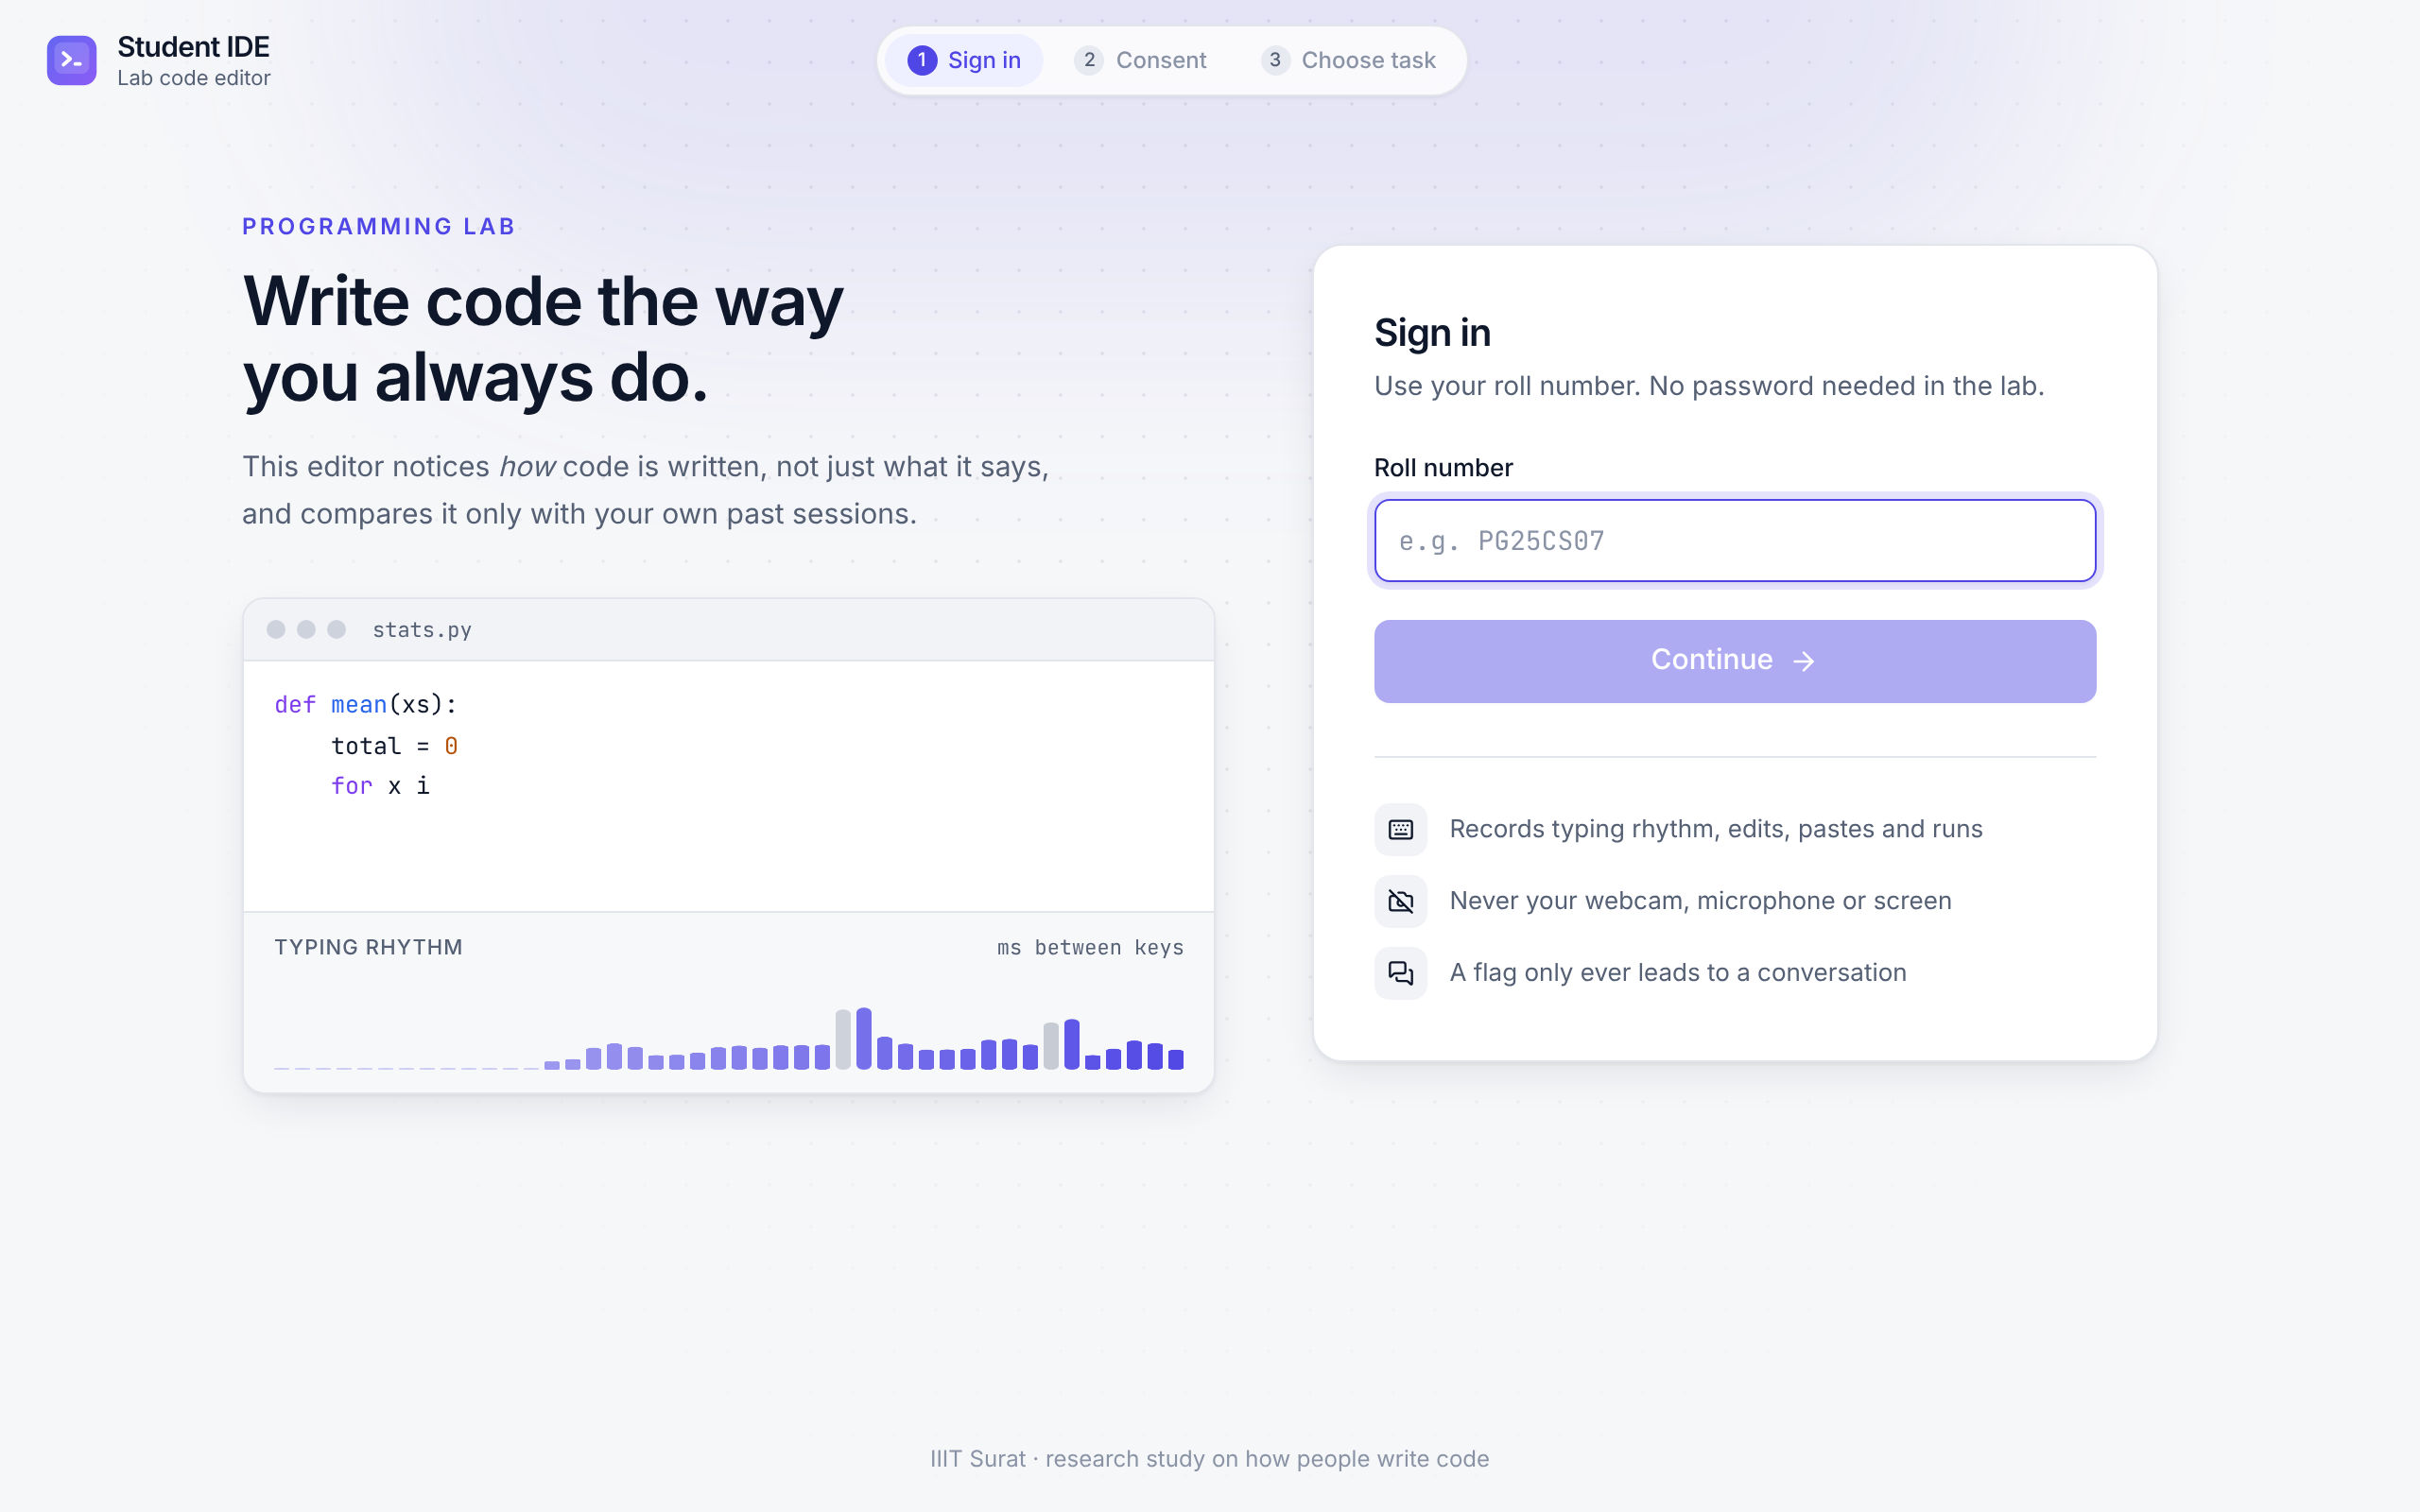
\includegraphics[width=\linewidth]{ui-redesign/after-light-01-login}
    \caption{Sign-in with the keystroke-rhythm illustration}
  \end{subfigure}\hfill
  \begin{subfigure}{0.48\textwidth}
    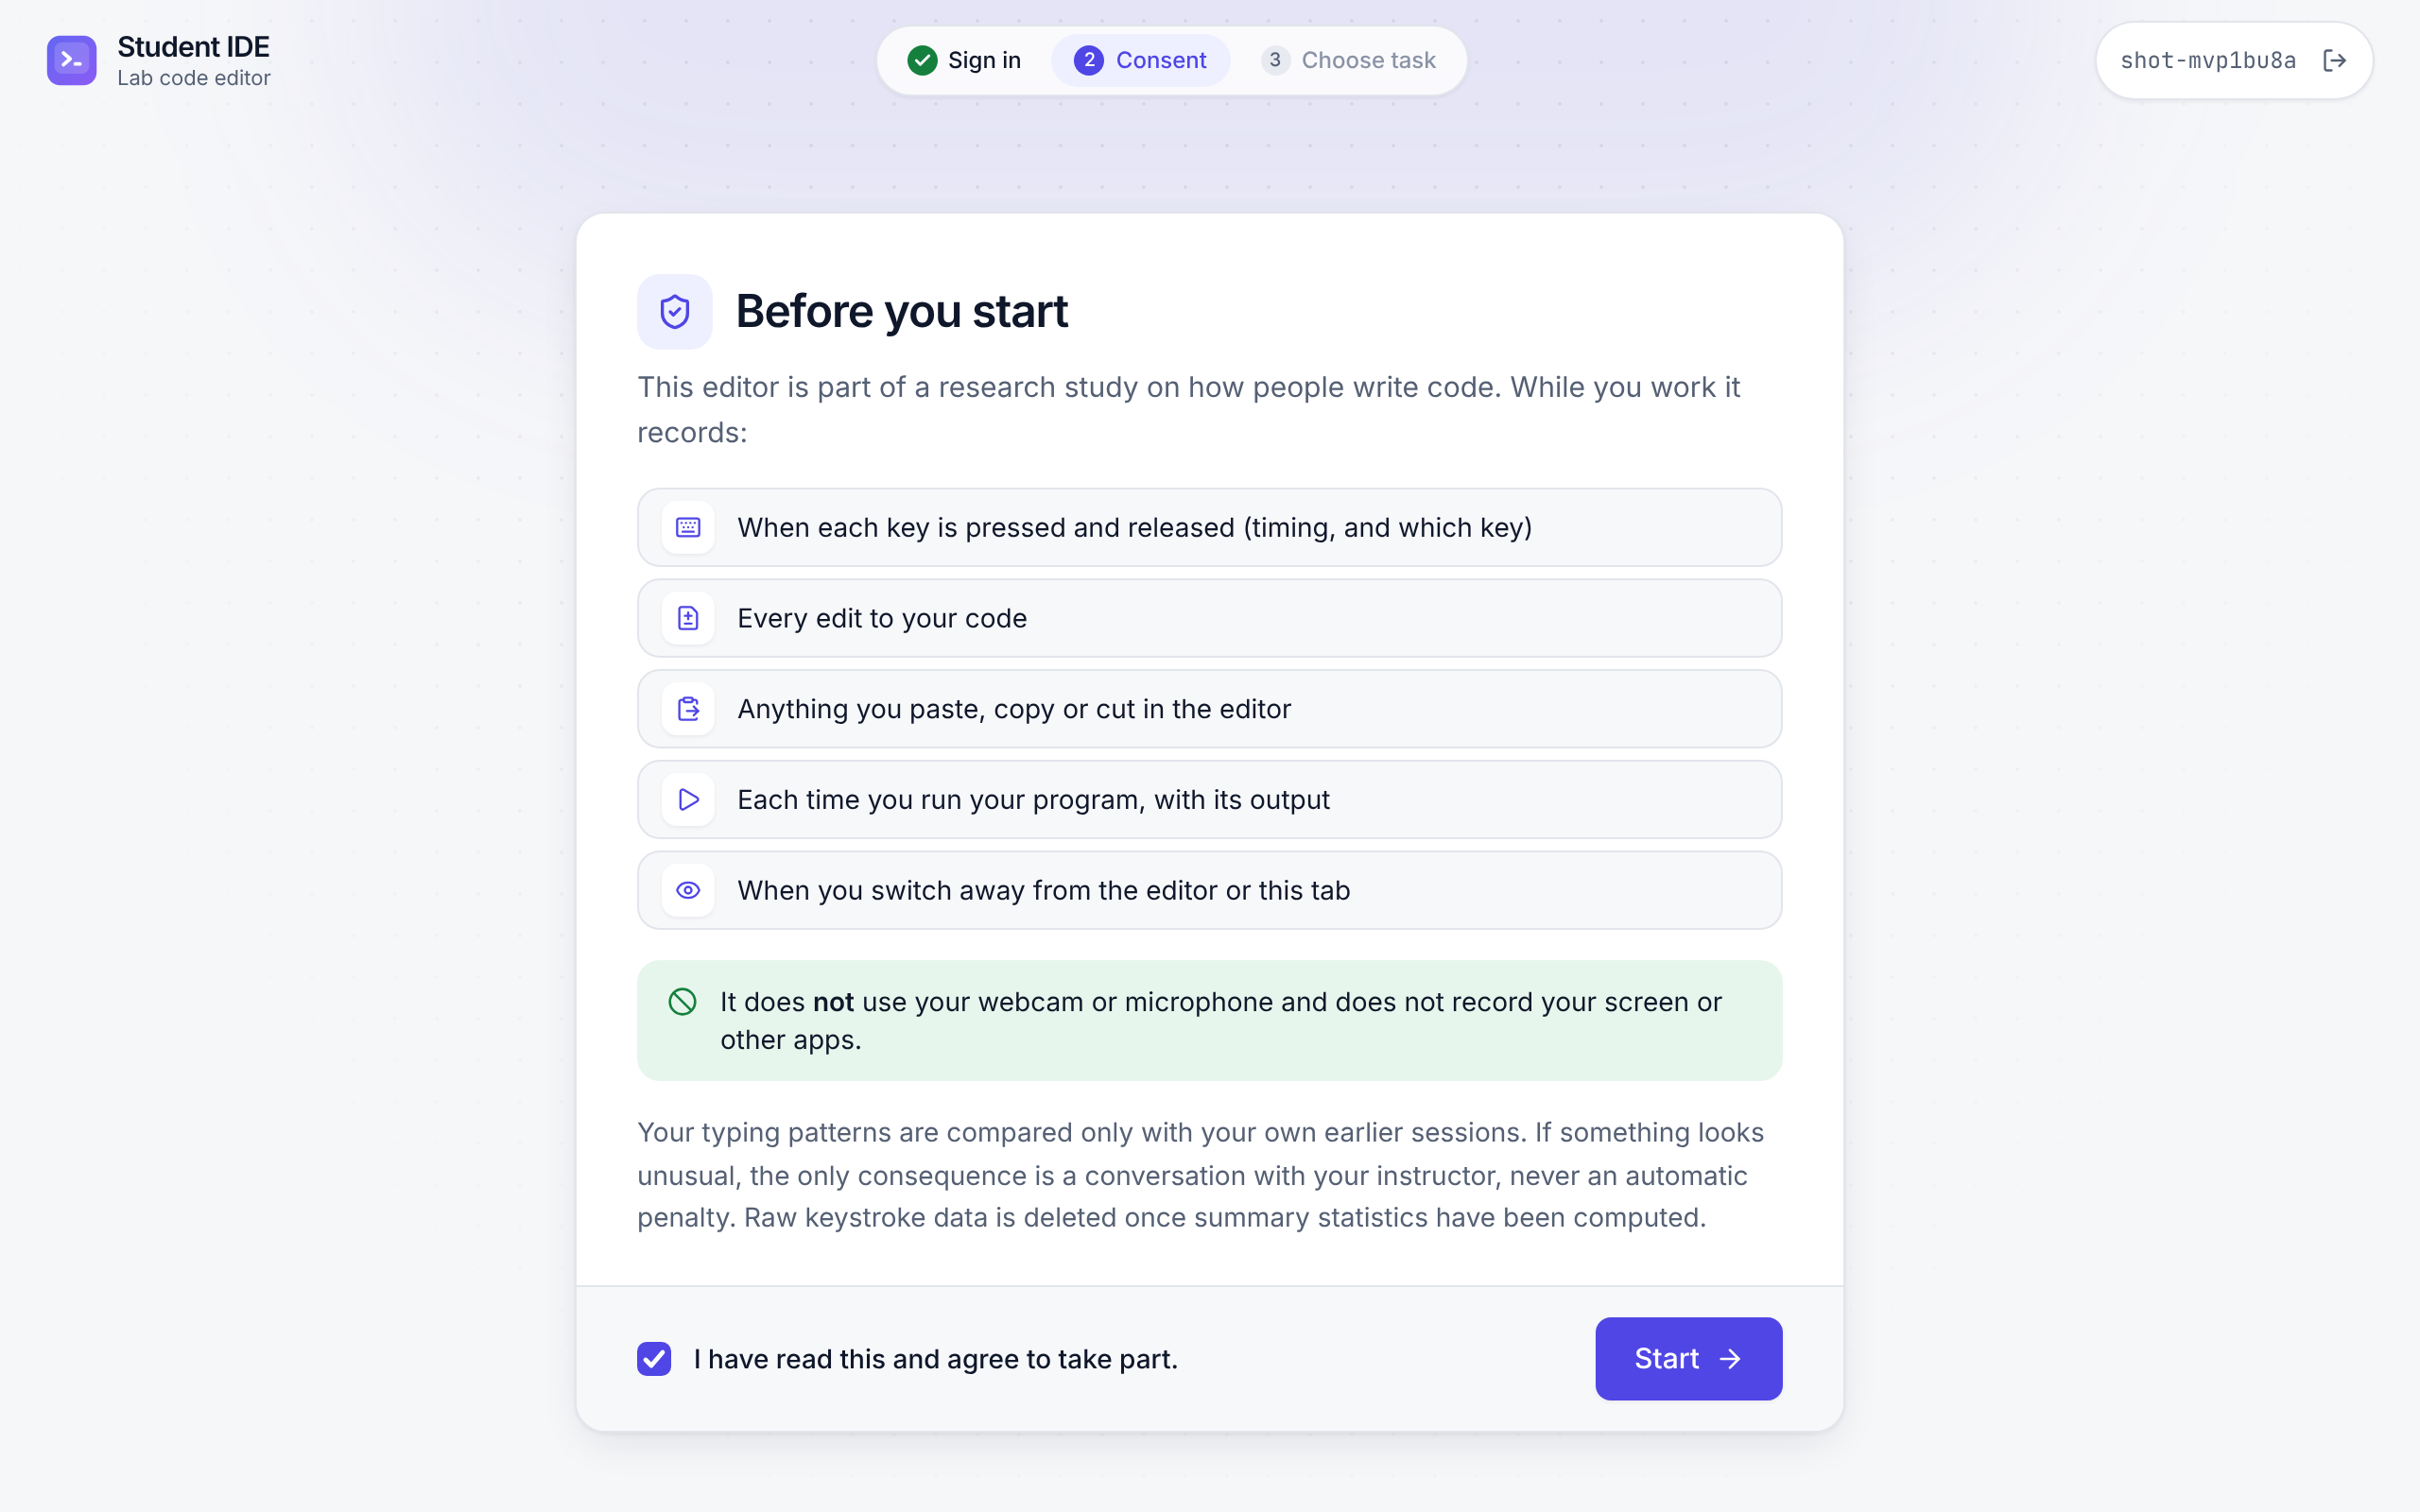
\includegraphics[width=\linewidth]{ui-redesign/after-light-02-consent}
    \caption{Consent notice}
  \end{subfigure}
  \caption{Student interface before and after the redesign. All screens,
  in light and dark themes, are in \texttt{snapshots/ui-redesign/}.}
  \label{fig:ui-before-after}
\end{figure}

\section{Event schema and storage}
\todo{Summary here, full schema in \cref{app:schema}.}

\section{Privacy and data lifecycle}
\todo{Raw keystrokes $\rightarrow$ baseline summary $\rightarrow$
deletion. Retention, consent, DPDP mapping.}

\section{Labs and questions}
\label{sec:teacher-authoring}
Teachers set up the sittings students record in from the same token-gated
area as the review timeline (\cref{fig:teach}). A \emph{lab} is one sitting,
such as a weekly lab class or one of the staged study sessions of
\cref{ch:study}. It holds ordered questions, each with a prompt, optional
starter code that opens in the editor and a sample input, and is assigned to
a roster of roll numbers or to everyone who signs in. A lab is a draft, open
(assigned students see it and can start) or closed (hidden, recordings kept).

Each recorded session stores the lab and question it answers, so every
keystroke, edit and run is tied to them through the session without changing
the event schema. The session also keeps a copy of the question as the
student saw it: a teacher may correct a prompt halfway through a lab, and an
older recording must still say what it was answering, which matters when
composing and transcribing are compared on the same question (RQ2). Labs and
questions with recordings can be closed or edited but not deleted. Because
each staged condition can be its own lab with its own roster, the condition
label of a study recording can come from the lab it was made in rather than
from a separate hand-kept list.

\begin{figure}[ht]
  \centering
  \begin{subfigure}{\textwidth}
    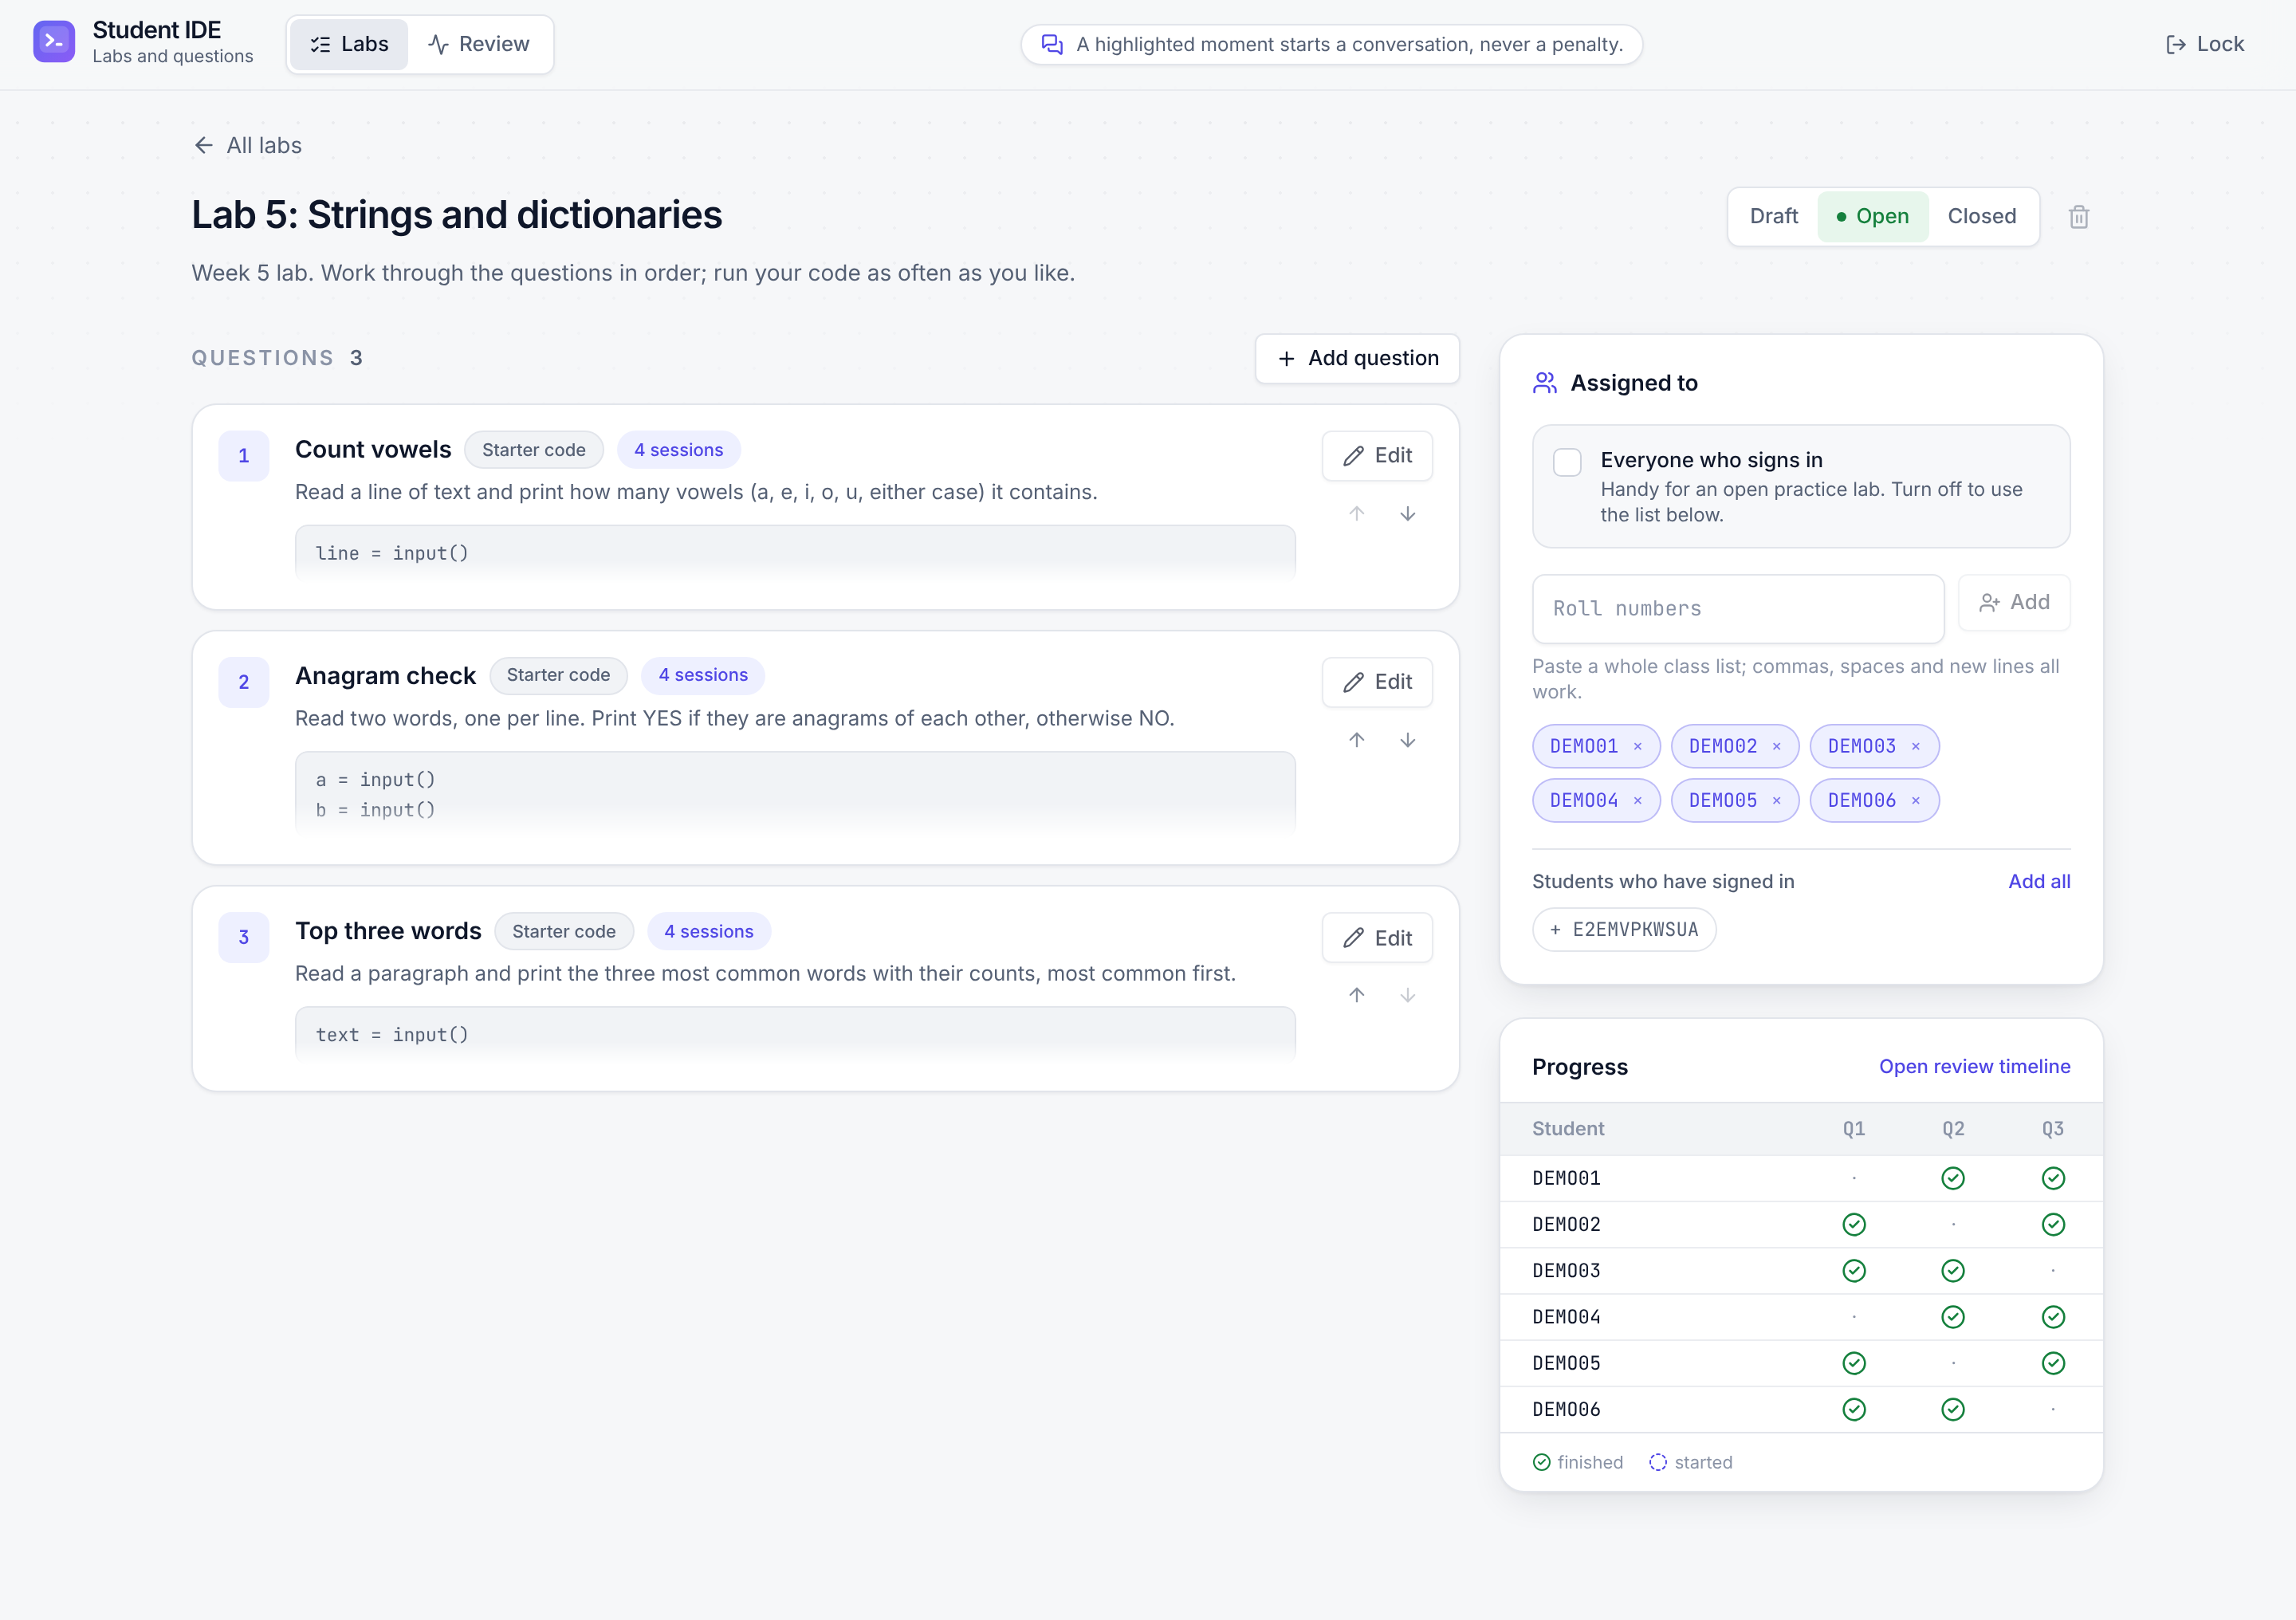
\includegraphics[width=\linewidth]{teach/teach-light-08-demo-lab}
    \caption{Teacher view of a lab: ordered questions with starter code, the
    roster, and who has started or finished each question.}
  \end{subfigure}\\[1ex]
  \begin{subfigure}{0.49\textwidth}
    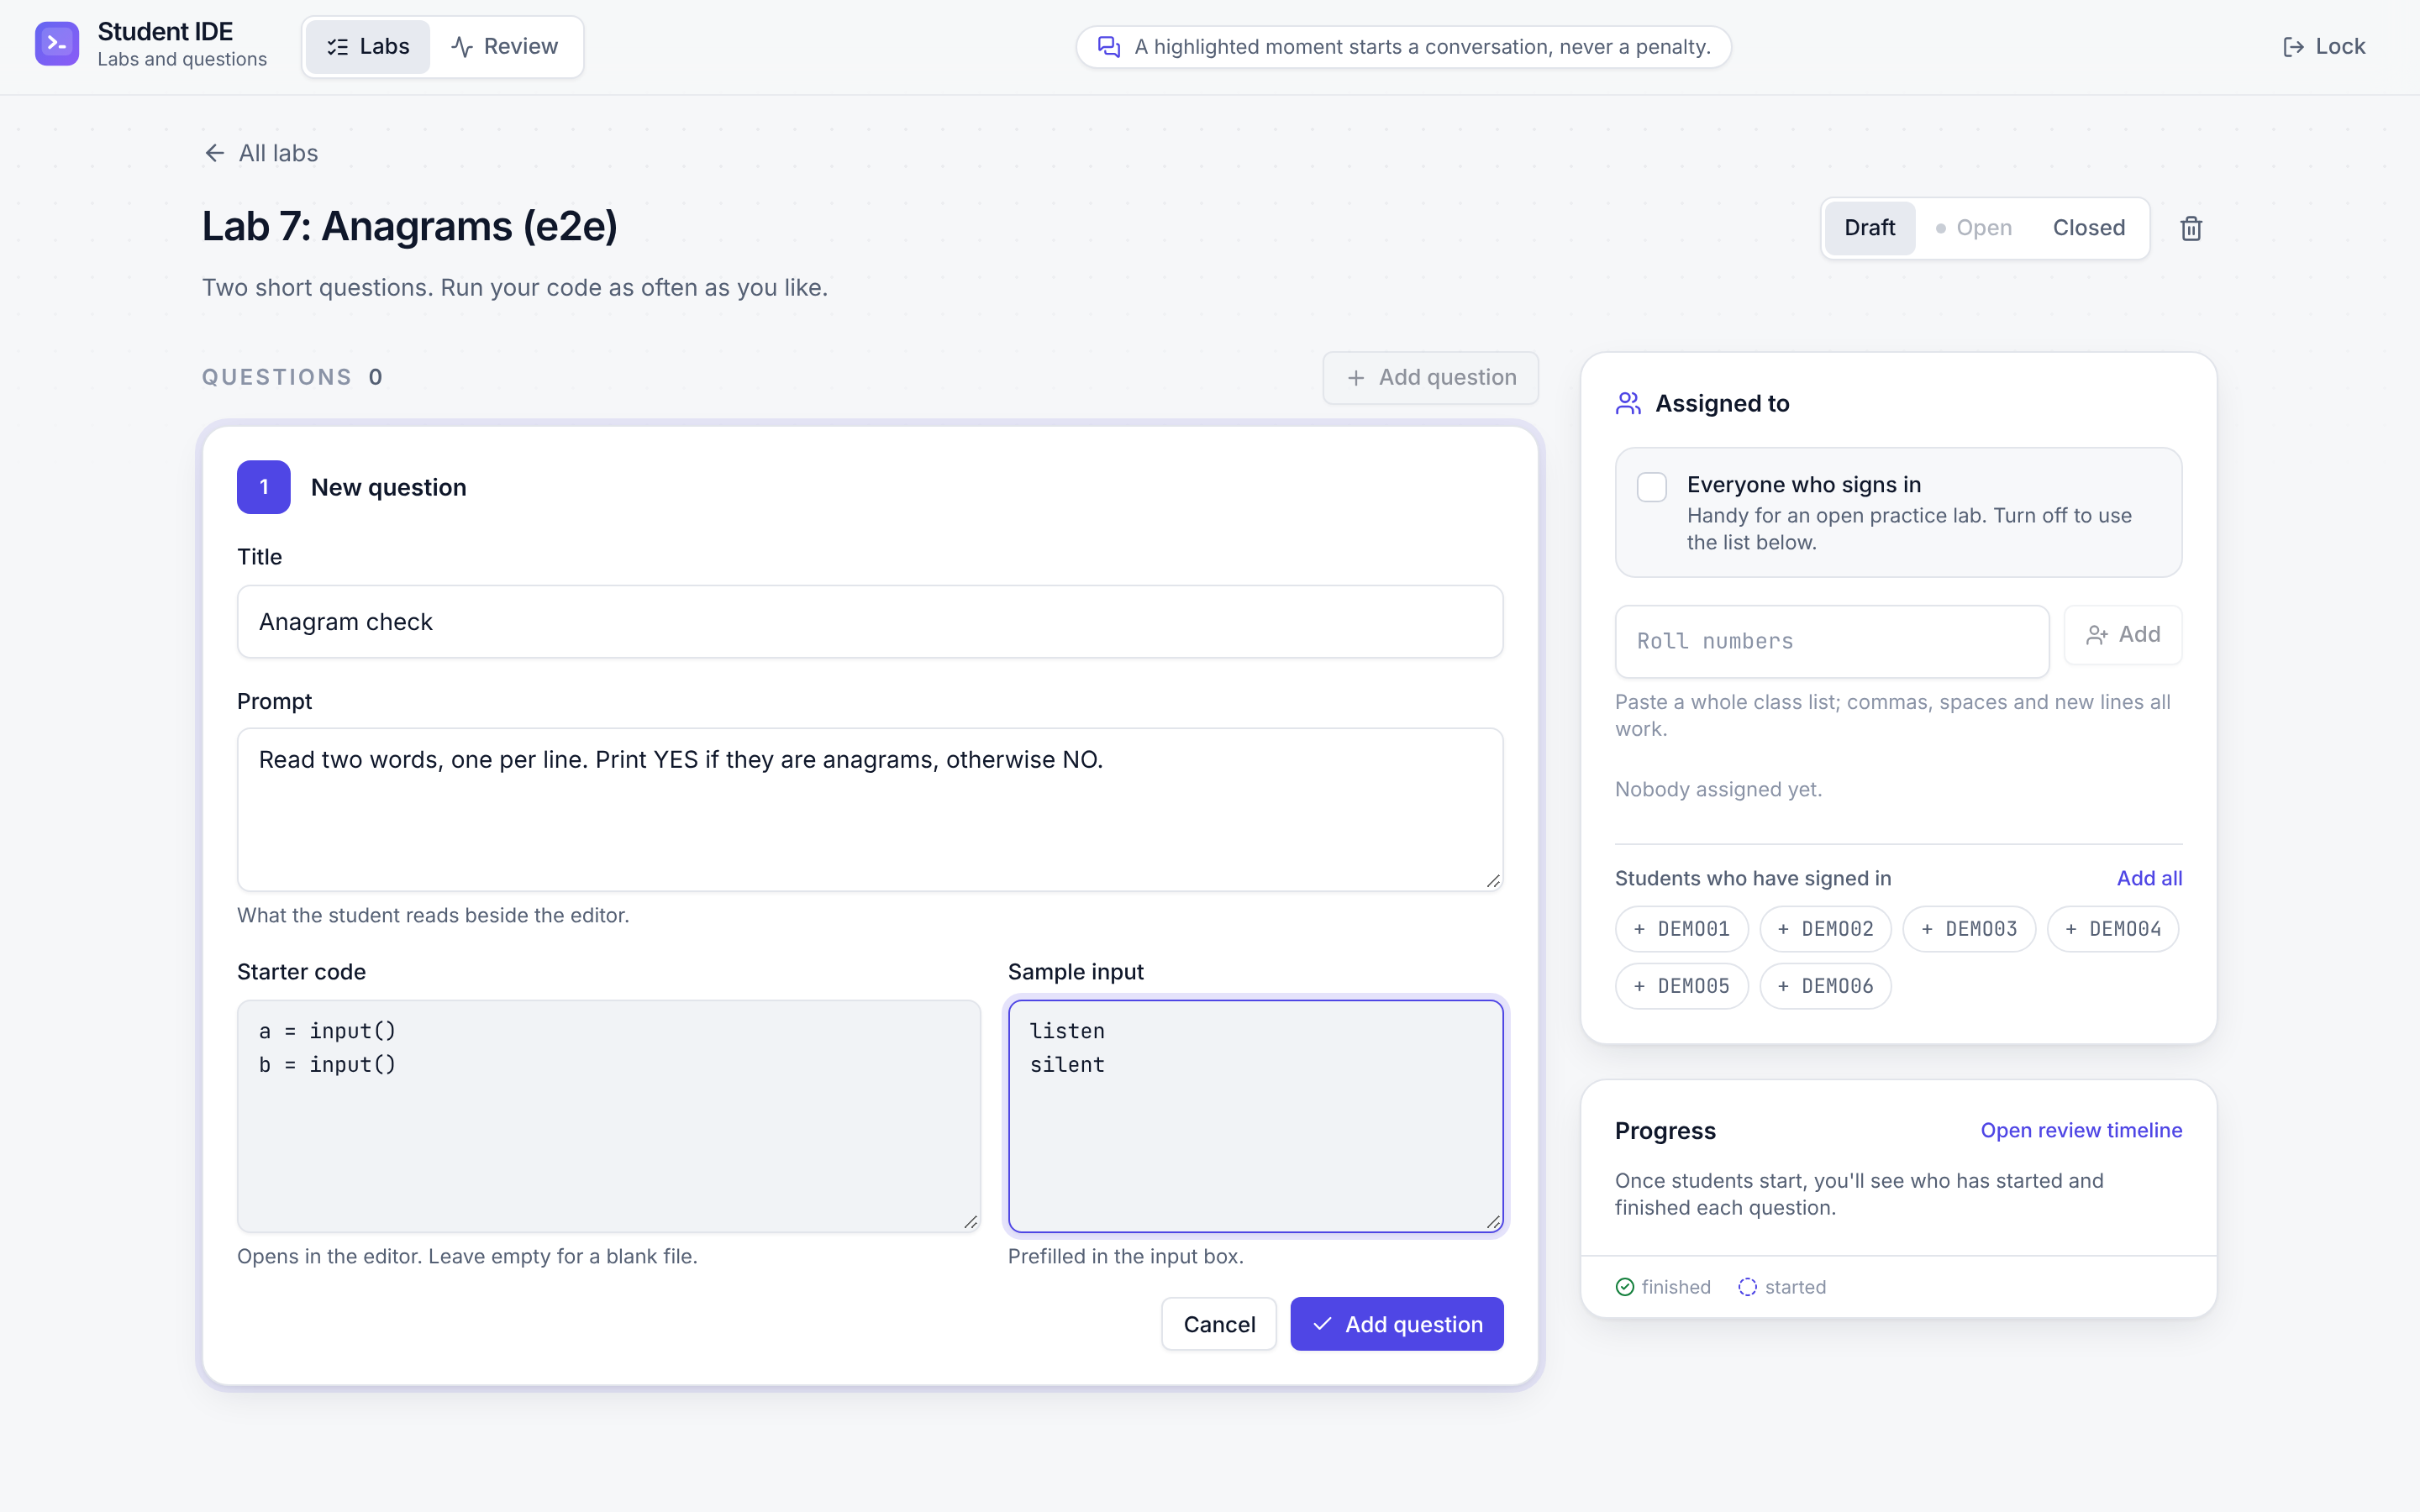
\includegraphics[width=\linewidth]{teach/teach-light-03-question-form}
    \caption{Adding a question.}
  \end{subfigure}\hfill
  \begin{subfigure}{0.49\textwidth}
    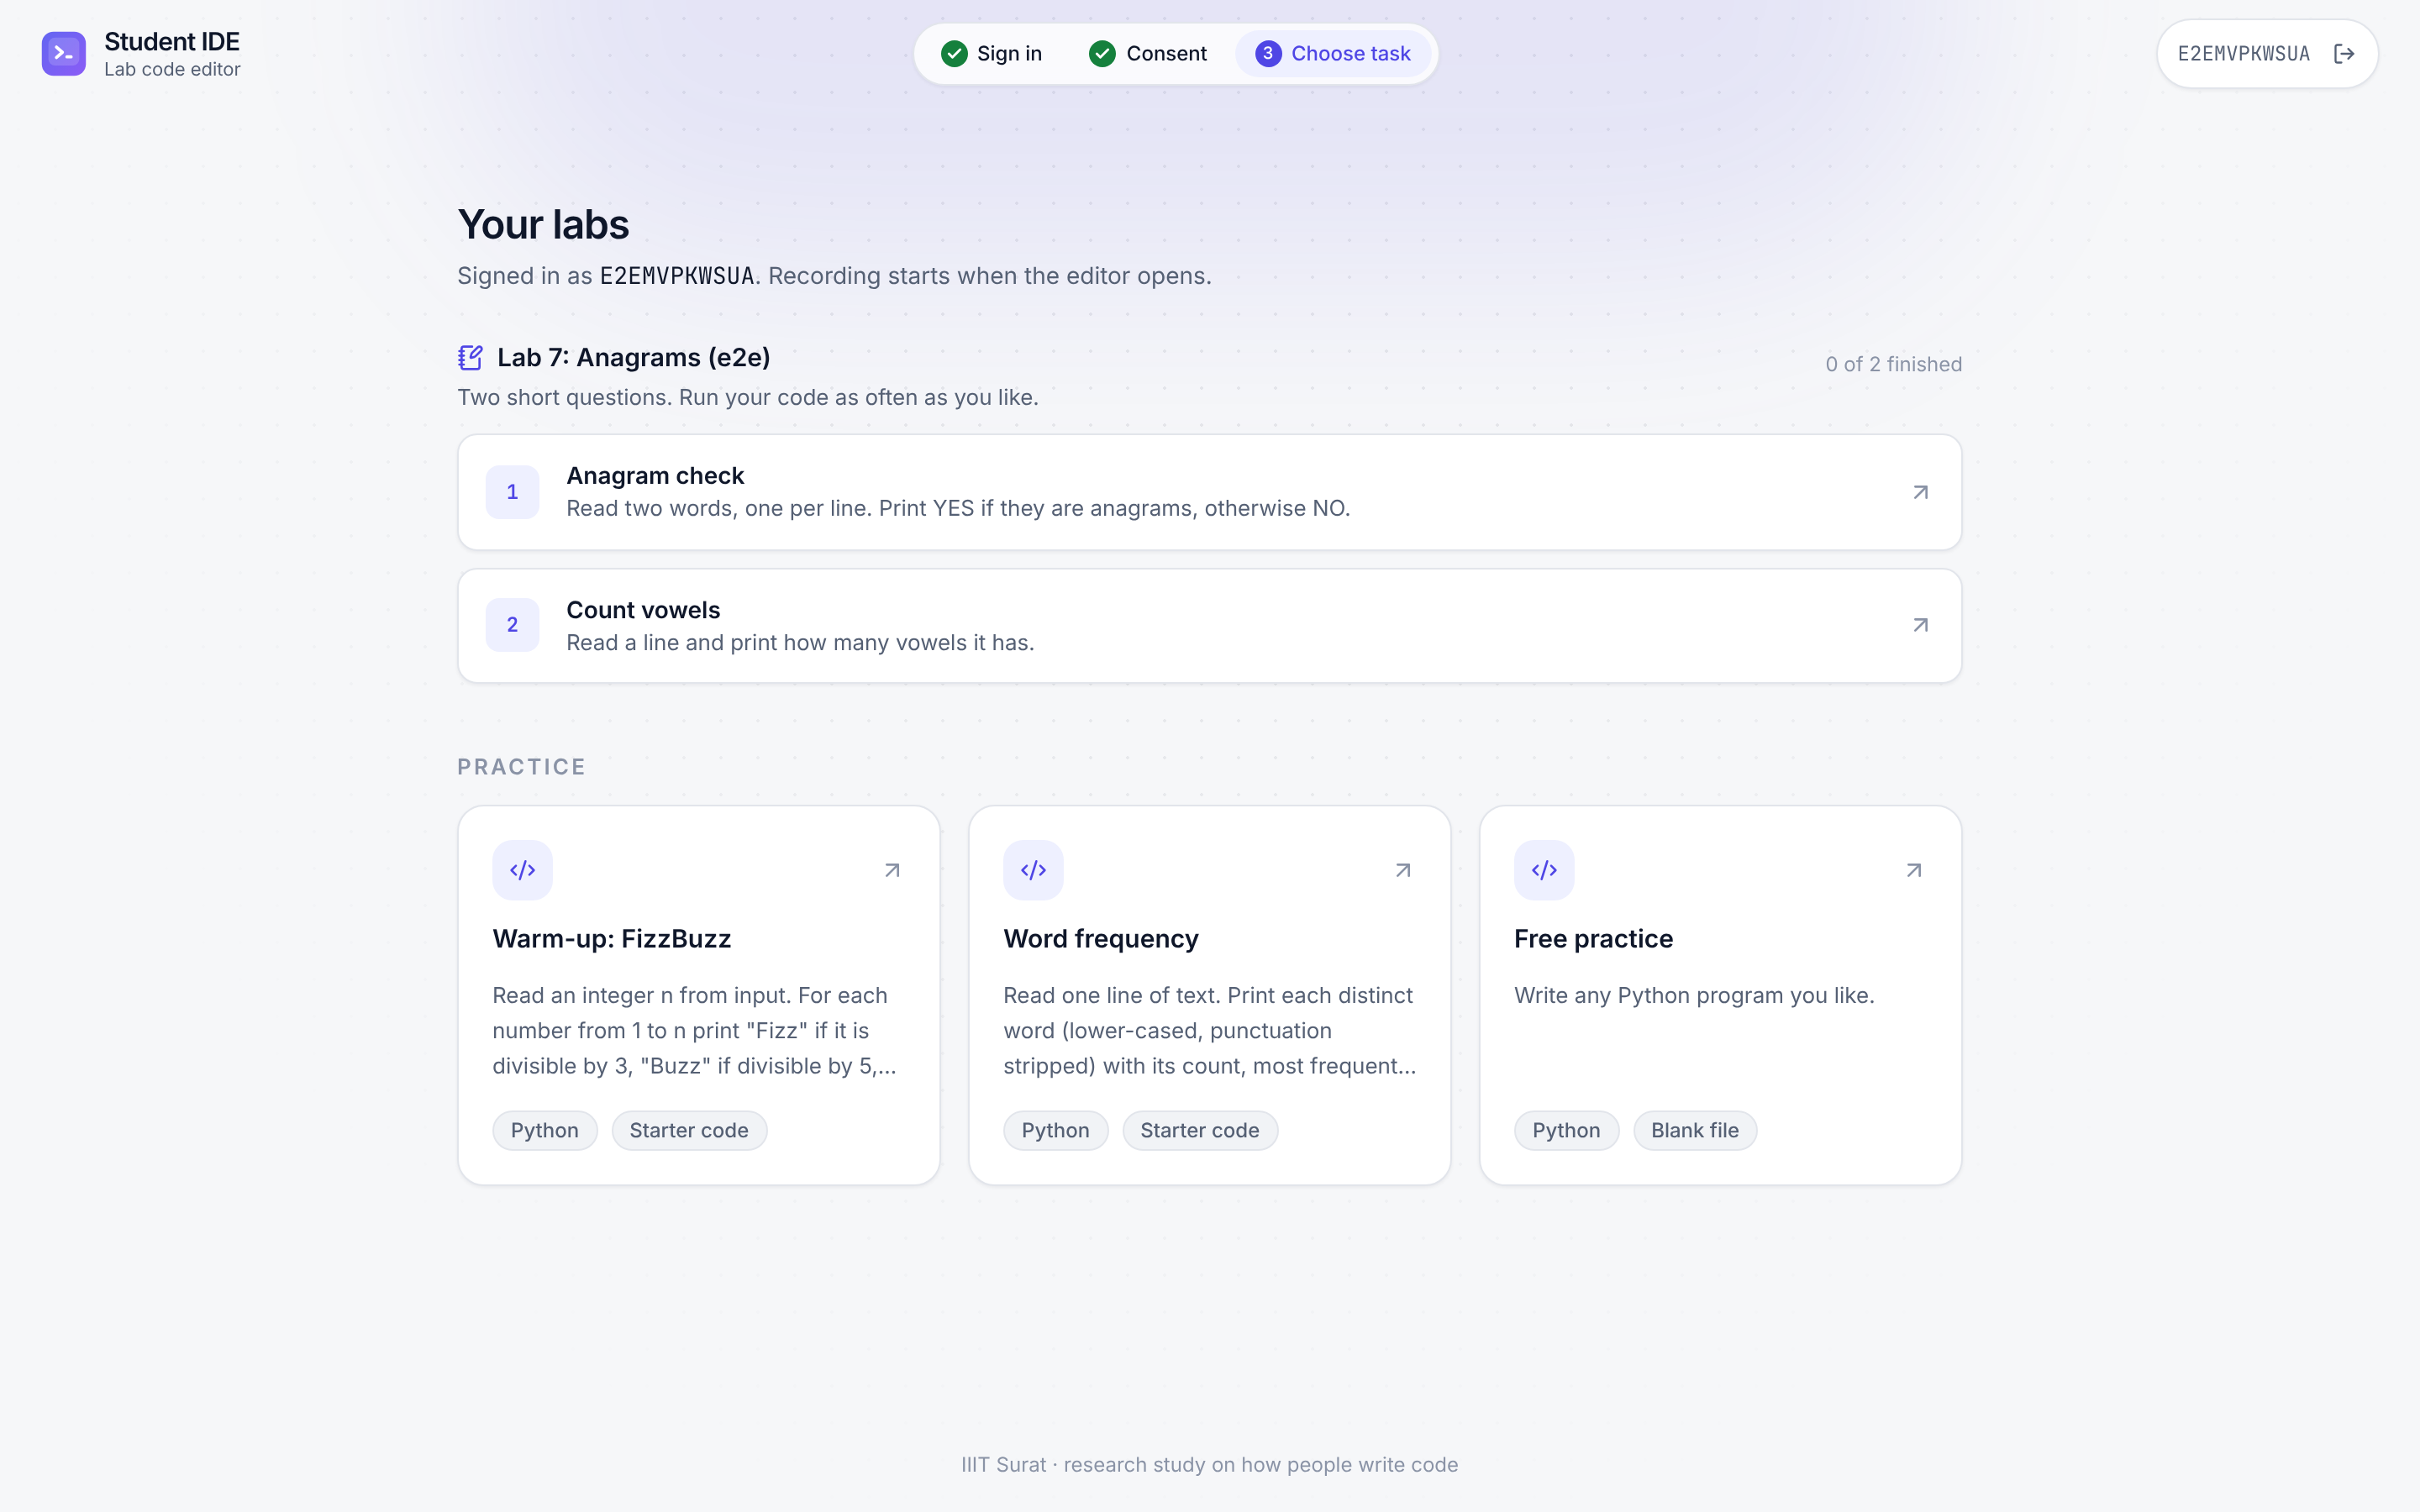
\includegraphics[width=\linewidth]{teach/teach-light-05-student-labs}
    \caption{What an assigned student sees after consent.}
  \end{subfigure}
  \caption{Labs and questions. Light and dark versions of every screen are
  in \texttt{snapshots/teach/}.}
  \label{fig:teach}
\end{figure}

\section{Class competitions}
\label{sec:competitions}
A competition is a lab run as a timed, class-wide challenge with a live
leaderboard (\cref{fig:compete}). It reuses the lab's questions, roster and
recorded sessions and adds a clock, a lobby in which students choose the name
shown on the board, and test-graded submissions. Ordinary labs treat
correctness as optional, since in class the effort is what matters; a
competition is the one place where correctness is scored. Every competition
question therefore needs at least one test case before the clock can start.
A submission earns $100 \times$ the share of tests passed, keeping the best
submission per question, plus up to 50 points for a full solve, scaled by the
share of the planned time still left. Wrong submissions cost nothing.

The board is kept deliberately gentle: by default students see the top ten
and their own place, never who is last; badges (first to solve, fastest per
question, solved them all, most bugs fixed) let more students stand out; and
only chosen board names are shown. The leaderboard reads nothing from the
detector or the review timeline, so a moment flagged for conversation can
never cost a place or become public. Competition sittings are recorded like
any lab; whether their time pressure changes typing enough to exclude them
from a student's baseline is left to the Phase~1 data.

\begin{figure}[ht]
  \centering
  \begin{subfigure}{0.49\textwidth}
    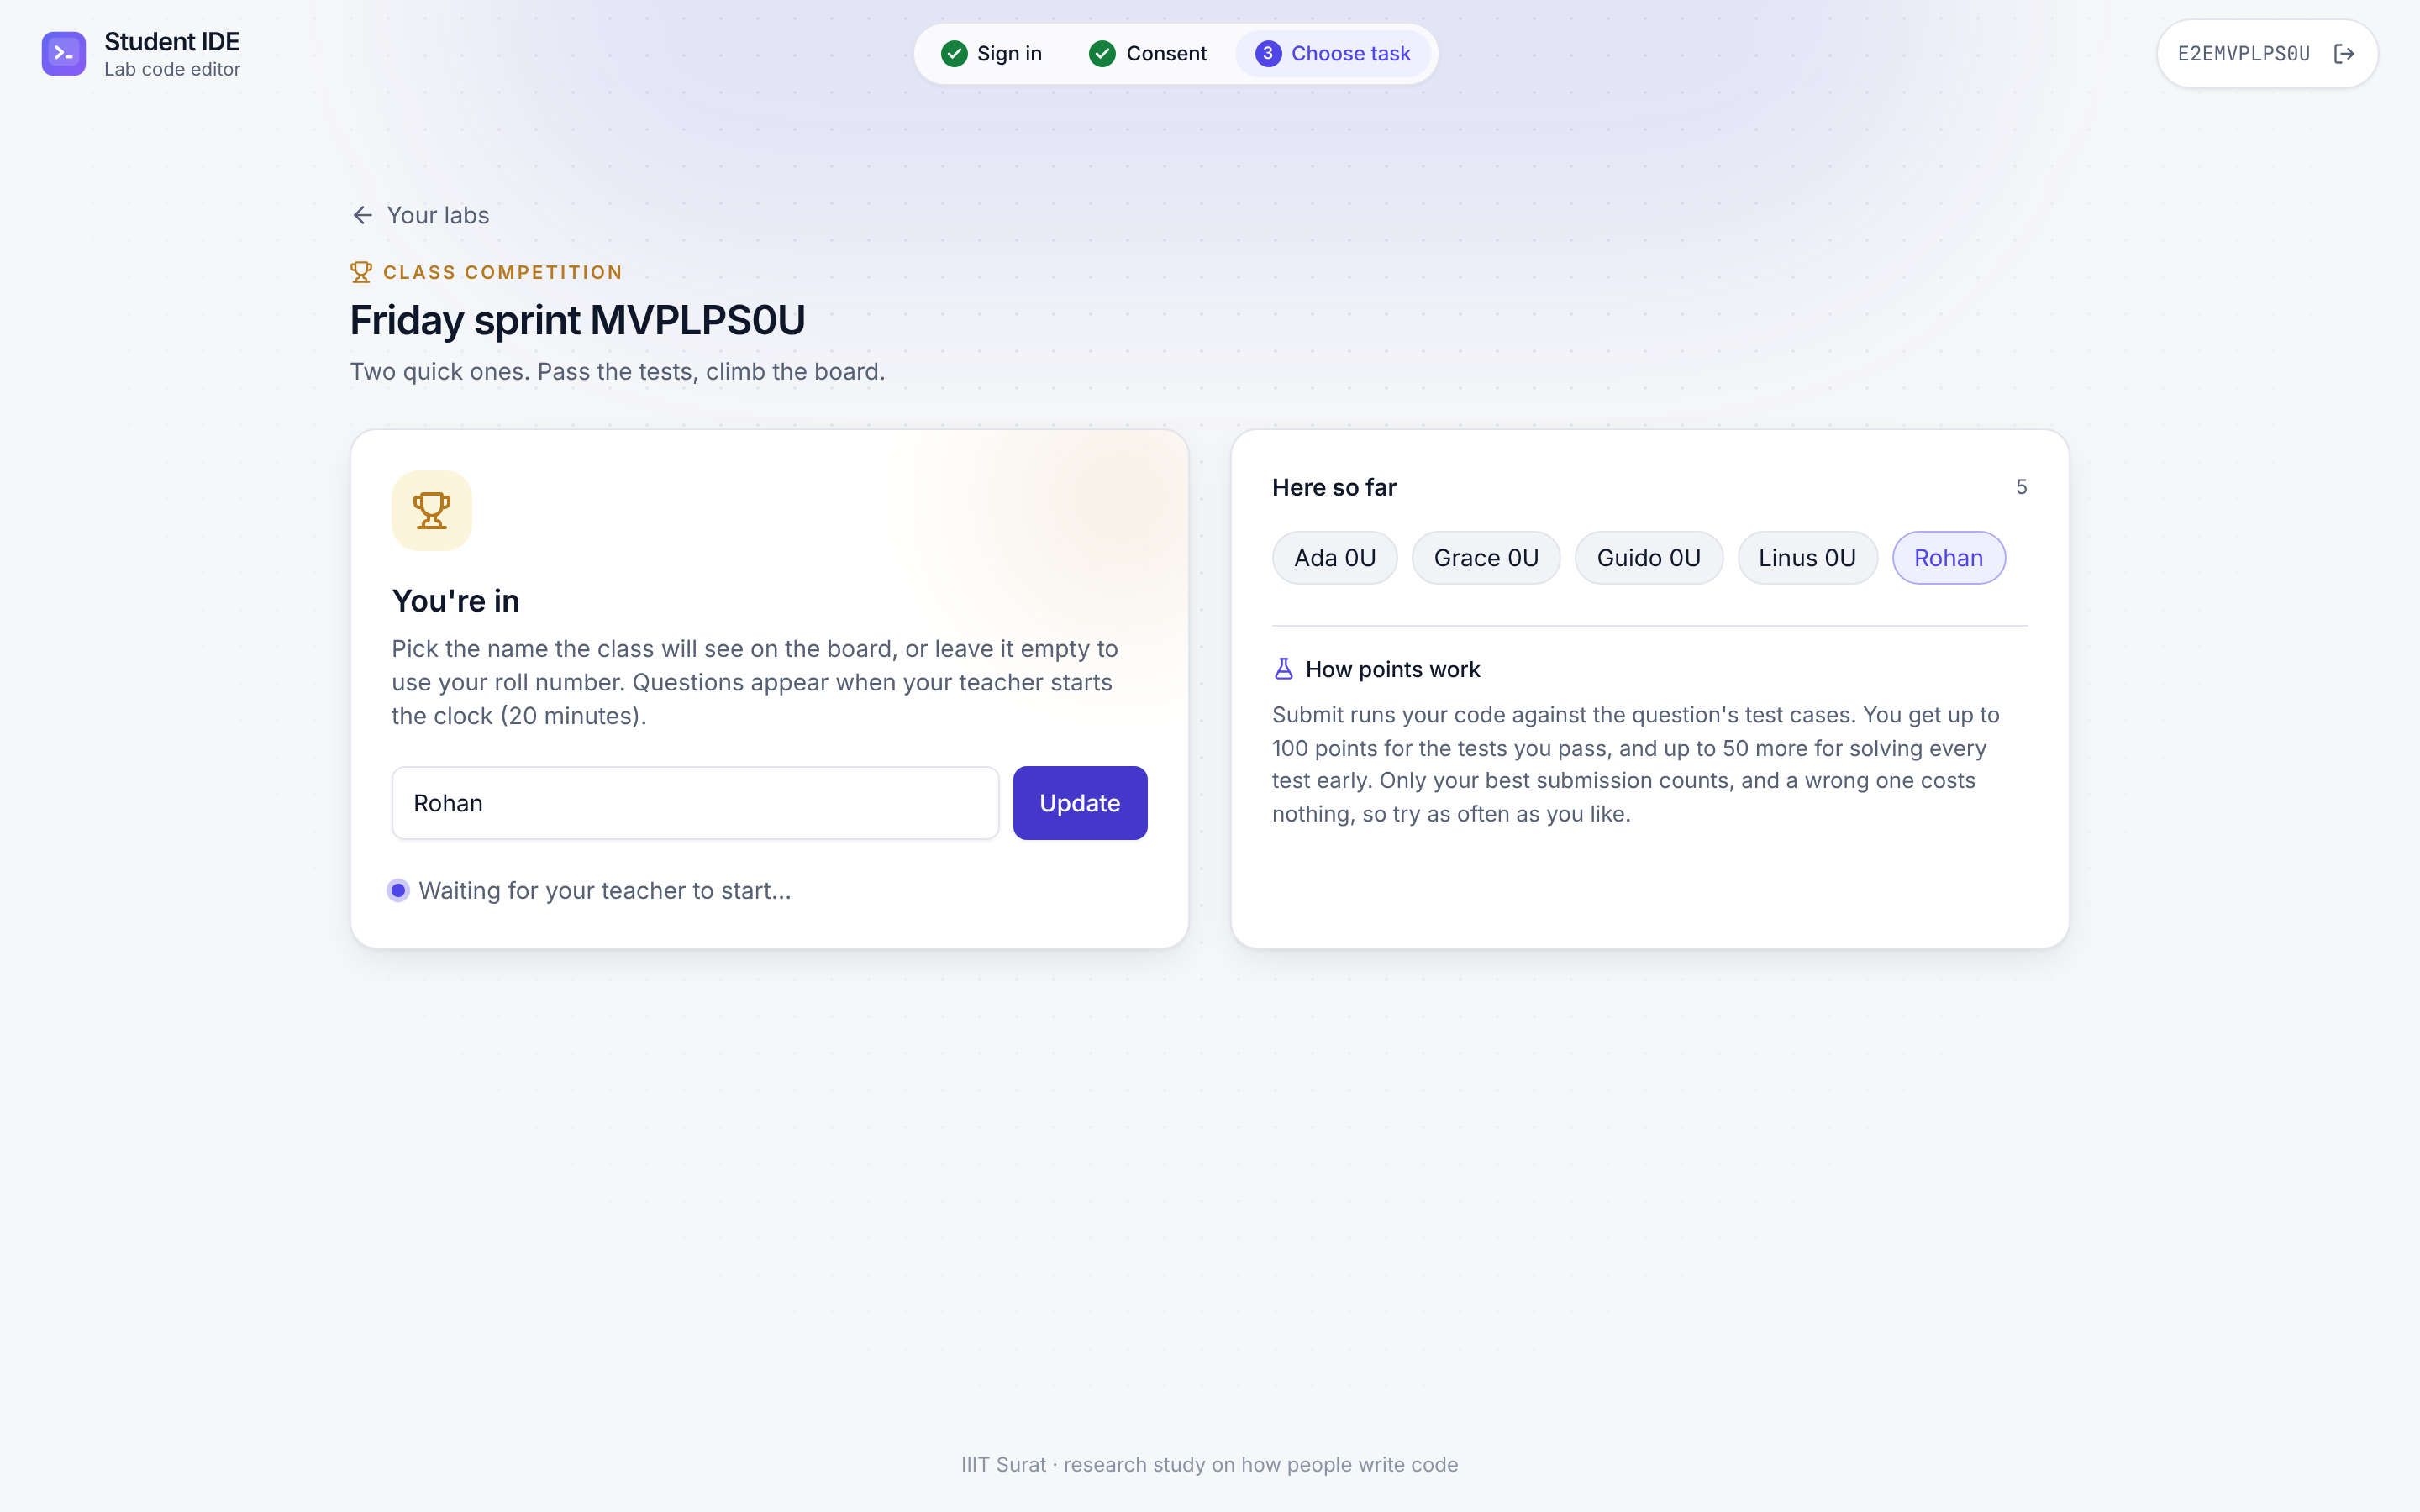
\includegraphics[width=\linewidth]{compete/compete-light-04-lobby}
    \caption{Lobby: students pick a board name before the clock starts.}
  \end{subfigure}\hfill
  \begin{subfigure}{0.49\textwidth}
    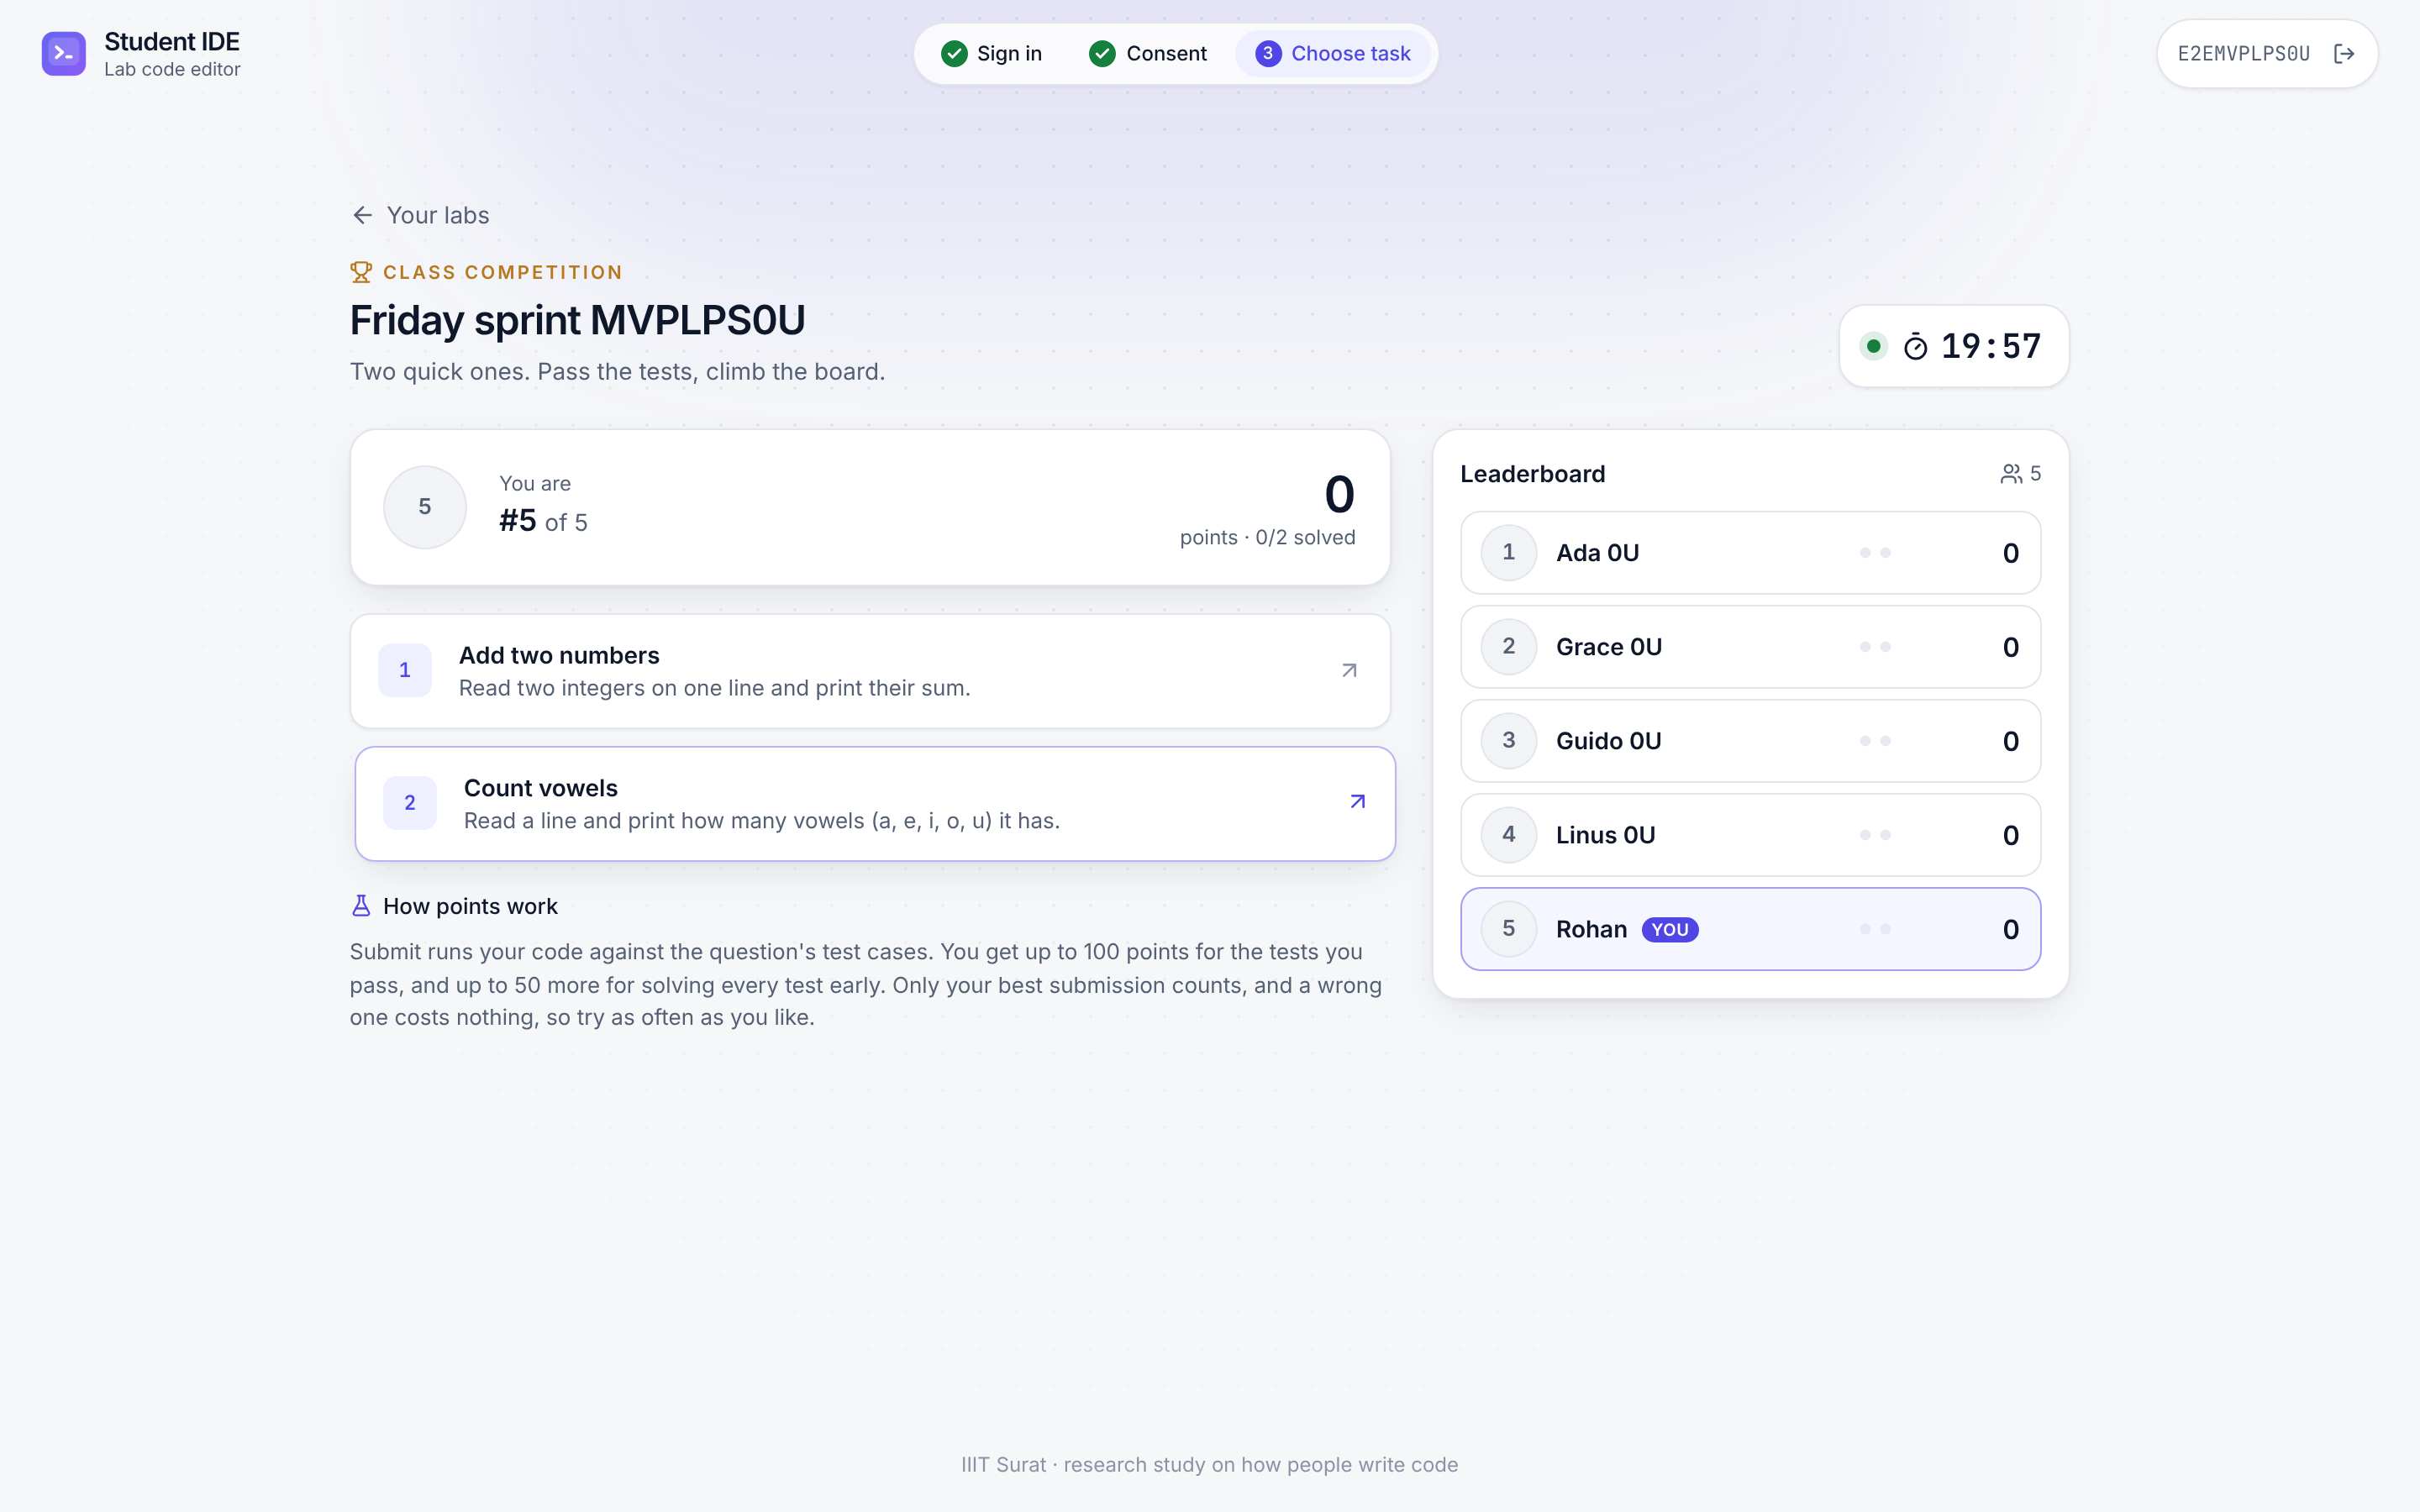
\includegraphics[width=\linewidth]{compete/compete-light-05-arena-live}
    \caption{Live: questions, own standing and the board.}
  \end{subfigure}\\[1ex]
  \begin{subfigure}{0.49\textwidth}
    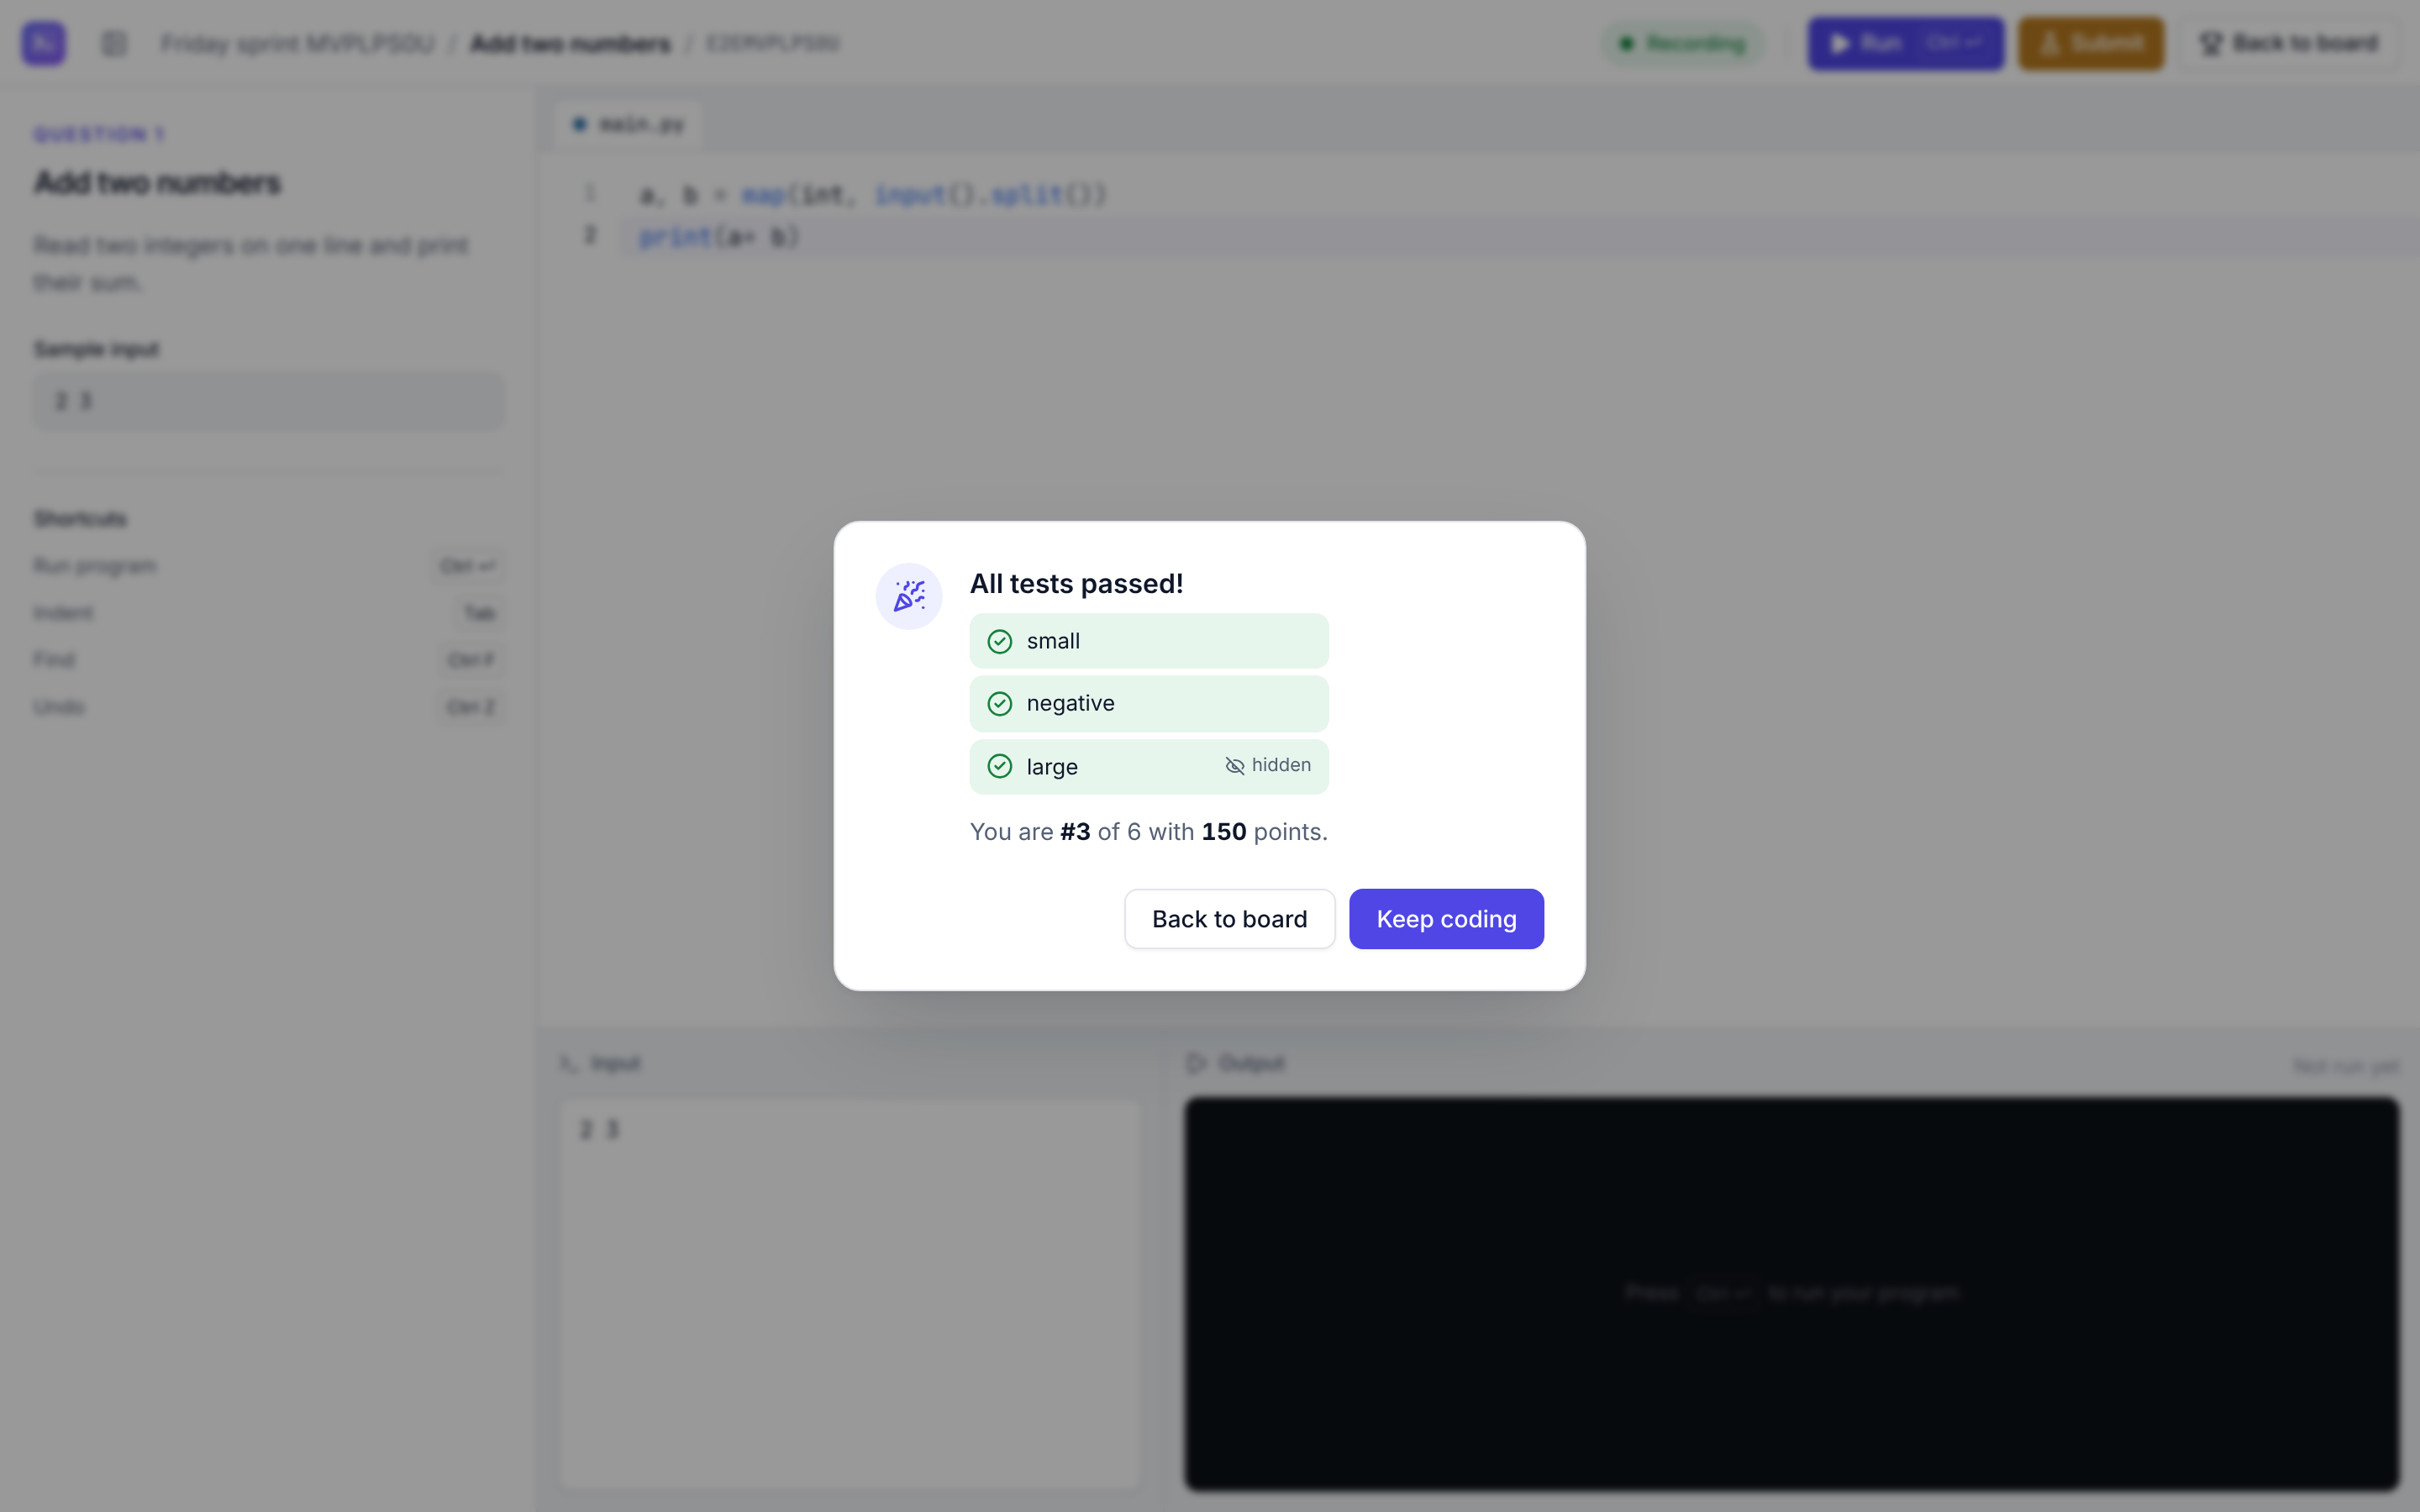
\includegraphics[width=\linewidth]{compete/compete-light-07-submit-solved}
    \caption{Submit runs the tests; hidden tests report pass or fail only.}
  \end{subfigure}\hfill
  \begin{subfigure}{0.49\textwidth}
    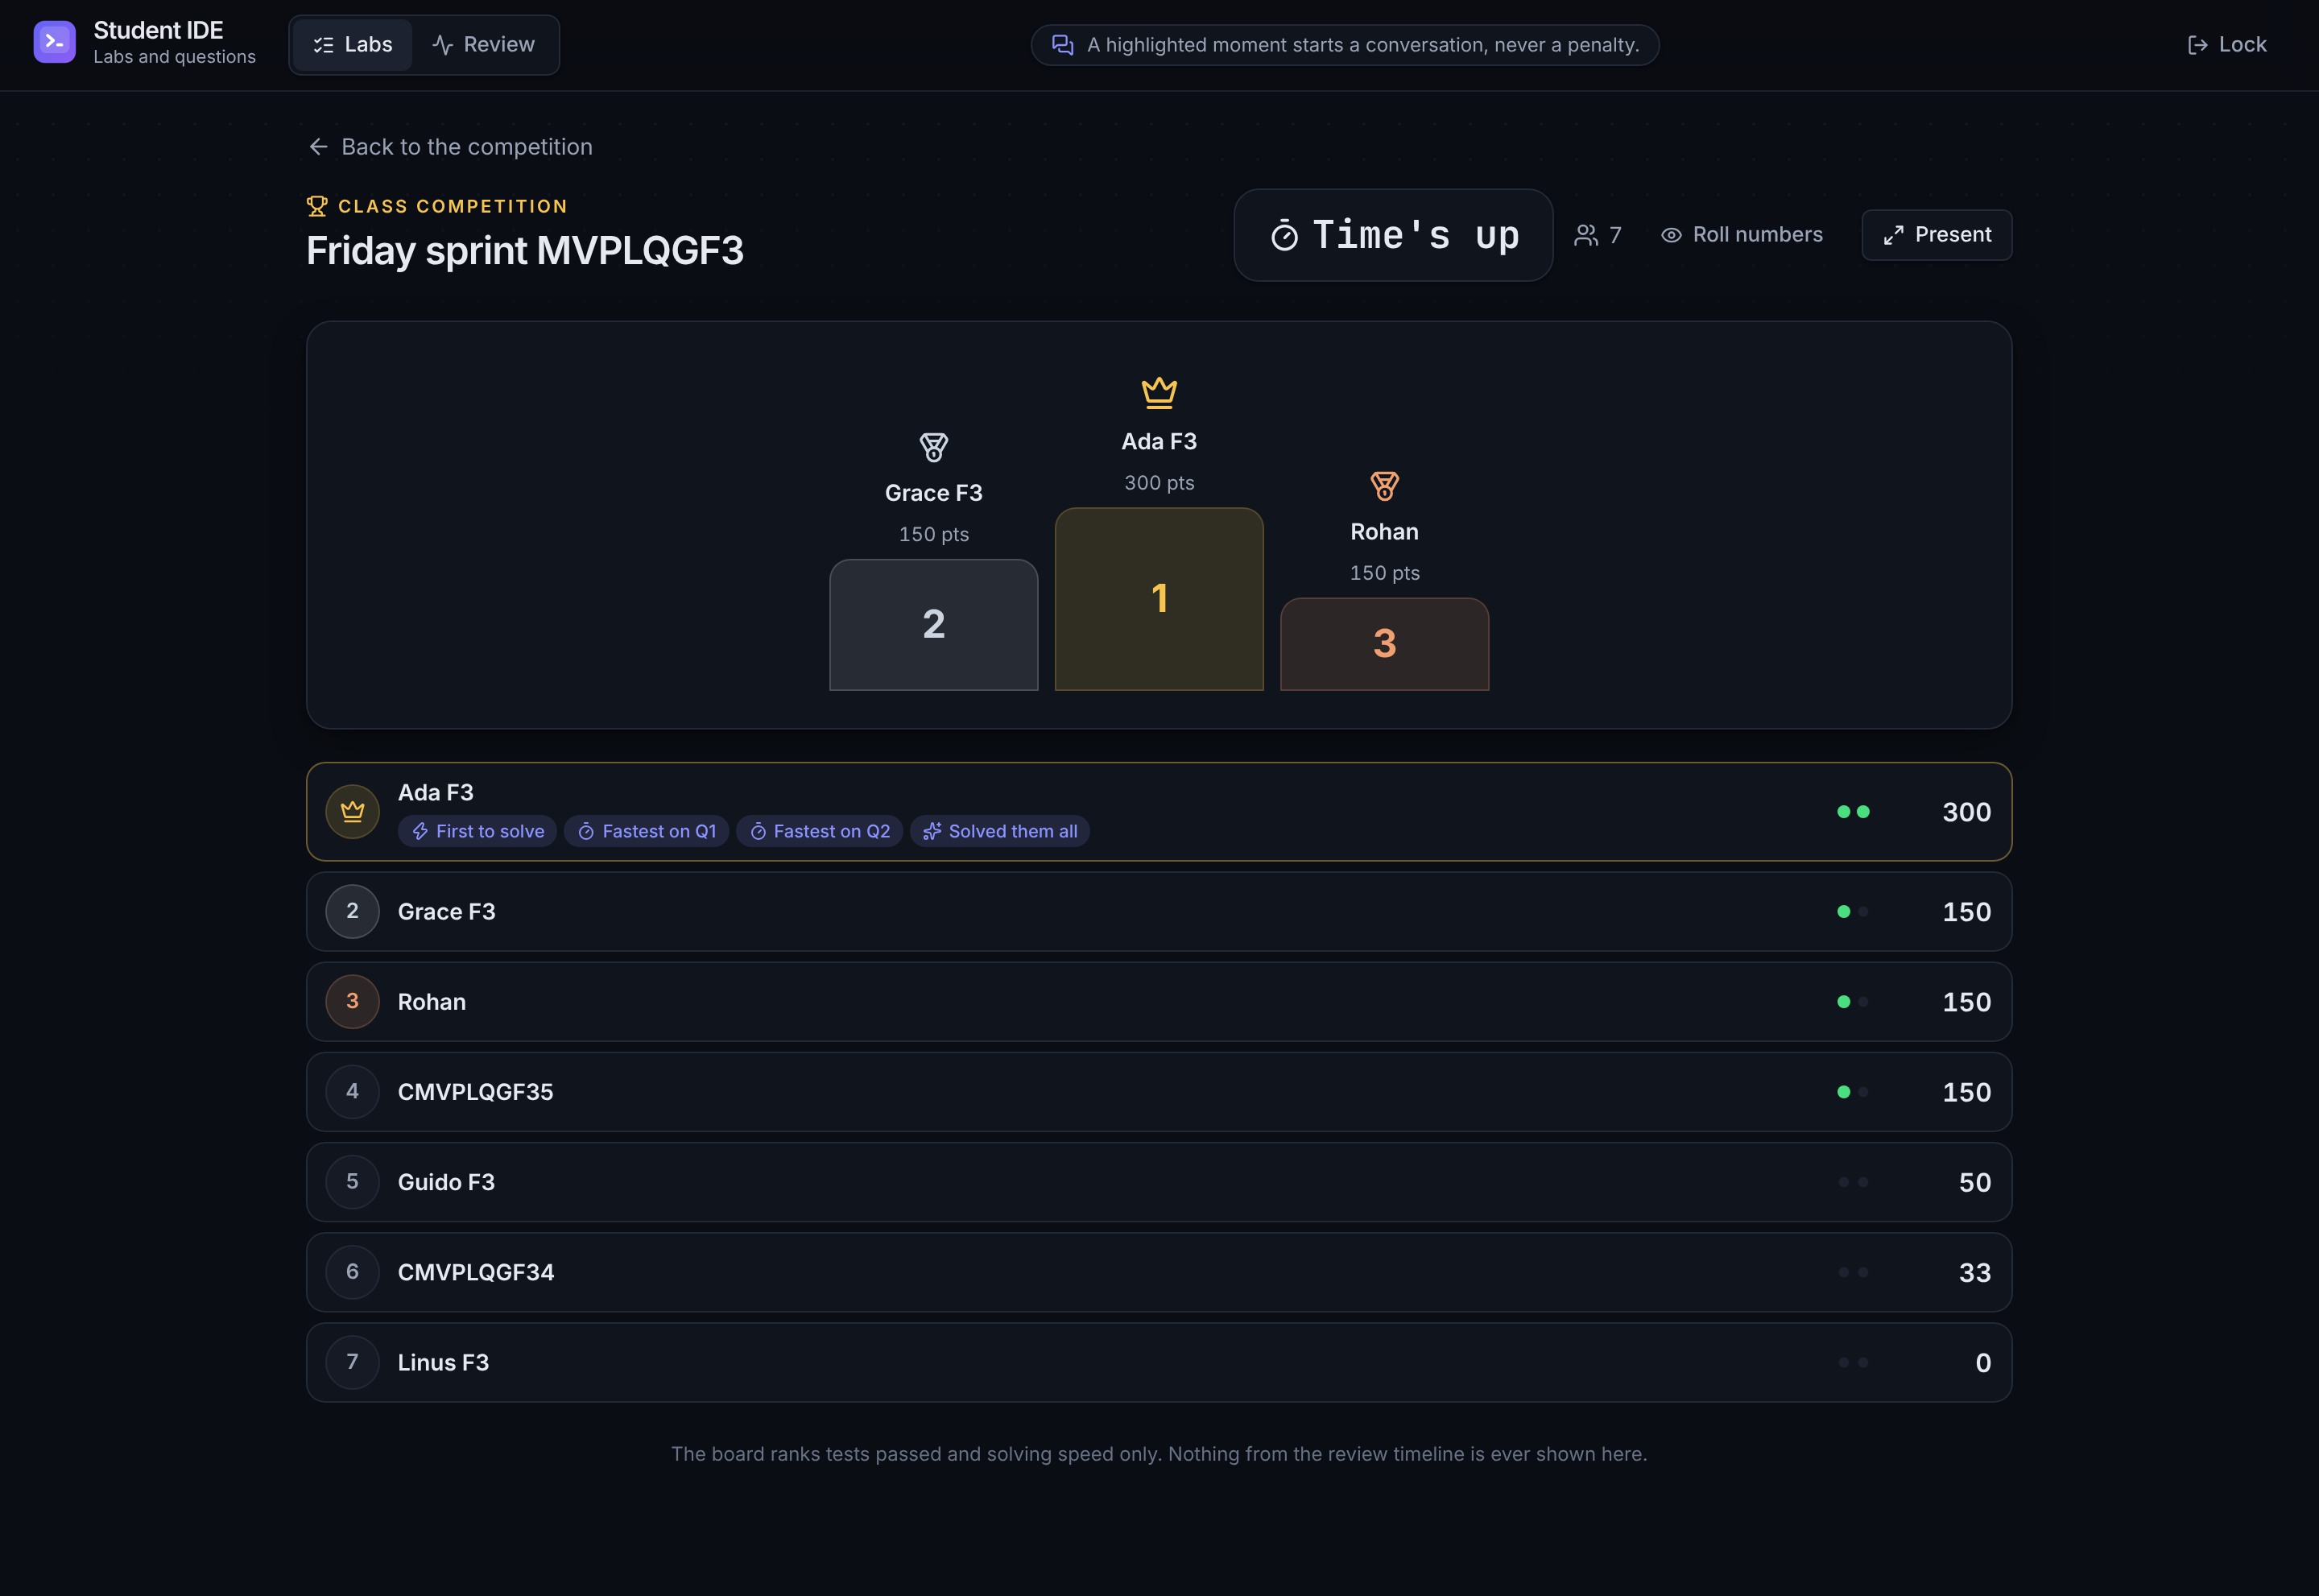
\includegraphics[width=\linewidth]{compete/compete-dark-09-podium}
    \caption{Teacher's projector board with the podium at the end.}
  \end{subfigure}
  \caption{Class competitions. All screens, light and dark, are in
  \texttt{snapshots/compete/}.}
  \label{fig:compete}
\end{figure}

\section{Teacher evidence timeline}
\label{sec:review-timeline}
The last part of the pipeline is a review screen for the teacher or
interviewer (\cref{fig:review-session}). It is opened from the same web
application under \texttt{\#/review}, but only with the research token
that also guards the raw-data API; without the token on the server the
whole review side is switched off. The token is kept in the browser tab
only.

\paragraph{What it shows.} An overview lists every session with a small
trace of both detector channels and the moments it found
(\cref{fig:review-overview}). Opening a session shows one time axis with,
from top to bottom: for each channel, a strip of per-window scores (how far
each \SI{30}{\second} window sits from the student's own baseline) and the
CUSUM trace drawn against its threshold; then pastes, times the student
left the editor, runs (clean or with an error) and typing activity. A
playhead can be dragged or played at 1--60$\times$; the code is rebuilt in
the browser from the recorded edits at that instant, with lines changed in
the previous \SI{30}{\second} tinted, and a strip of the last key-press
intervals shows the typing rhythm at that point. The replay was checked
against all 524 stored snapshots of eight sessions with no mismatch.

\paragraph{From alarms to moments.} CUSUM restarts after every alarm, so a
lasting change (for example, a second person typing for the rest of the
session) raises a chain of alarms, each starting where the previous one
fired. The screen merges such a chain into one \emph{moment to discuss},
with the detector's estimated start, the time it was first noticed and how
long the difference lasted. For each moment it lists the habits that moved
most between the estimated start and the first alarm, in the student's own
units (``time between keys: usual \SI{158}{\milli\second}, here
\SI{134}{\milli\second}'') with a bar for how many of the student's usual
spreads that is. These are the same per-feature $z$ values the detector
sums, so the explanation is the model rather than a story told about it.

\paragraph{Wording.} Nothing on the screen says ``flag'', ``cheating'' or
``suspicious''. A session either has \emph{moments worth a conversation}
or ``nothing stood out''. Every moment comes with three suggested
questions (walk me through this code; did anything change at that point;
make a small change while I watch) and the reminder that habits shift for
ordinary reasons and that no mark or penalty follows from the screen.
Baseline-week sessions are scored only against the student's other
baseline sessions and are labelled as a check of the baseline, not of the
student; students without enough baseline sessions are not scored at all.

\paragraph{The screen runs the evaluated detector.} The review screen reads
the configuration the evaluation harness froze
(\texttt{thesis/evaluation/frozen-config.json}, \cref{sec:rq1-harness}), so
what a teacher sees is what was evaluated: three lanes (typing rhythm and
key-pair timing on \SI{30}{\second} windows, way of working on
\SI{90}{\second} windows), each with its own CUSUM $k$, the population prior
for short baselines and the thresholds $h$ calibrated on the dev students.
Each lane is drawn on its own window grid against one time axis. The
population parts (feature weights, the key-pair vocabulary, the prior) are
fitted on the class's own baseline sessions once three students have one,
just as the harness fits them on its training students. Thresholds can be
overridden once they are calibrated on the class's real data.

\paragraph{Demo data.} \texttt{python -m studentide.seed} fills a fresh
database with simulated students (four honest baseline weeks, then
sessions under the study conditions). Their ground truth is stored with
the session and can be overlaid on the timeline
(\cref{fig:review-session}b), which made the screen testable before any
real student was recorded. It is refused on an existing database file so
demo and real data never mix. On the default demo (six simulated students,
twelve assessed sessions) with the frozen configuration, seven of the eight
non-honest sessions got a moment on the expected kind of lane (one
speed-matched takeover was missed), none of the four honest sessions did,
and none of the 24 baseline-week sessions did either (with the earlier
untuned thresholds and no prior, 5 of 24 baseline-week sessions had raised
a moment). This is a check that the screen shows the detector faithfully,
not an evaluation (that is \cref{ch:rq1}).

\begin{figure}[ht]
  \centering
  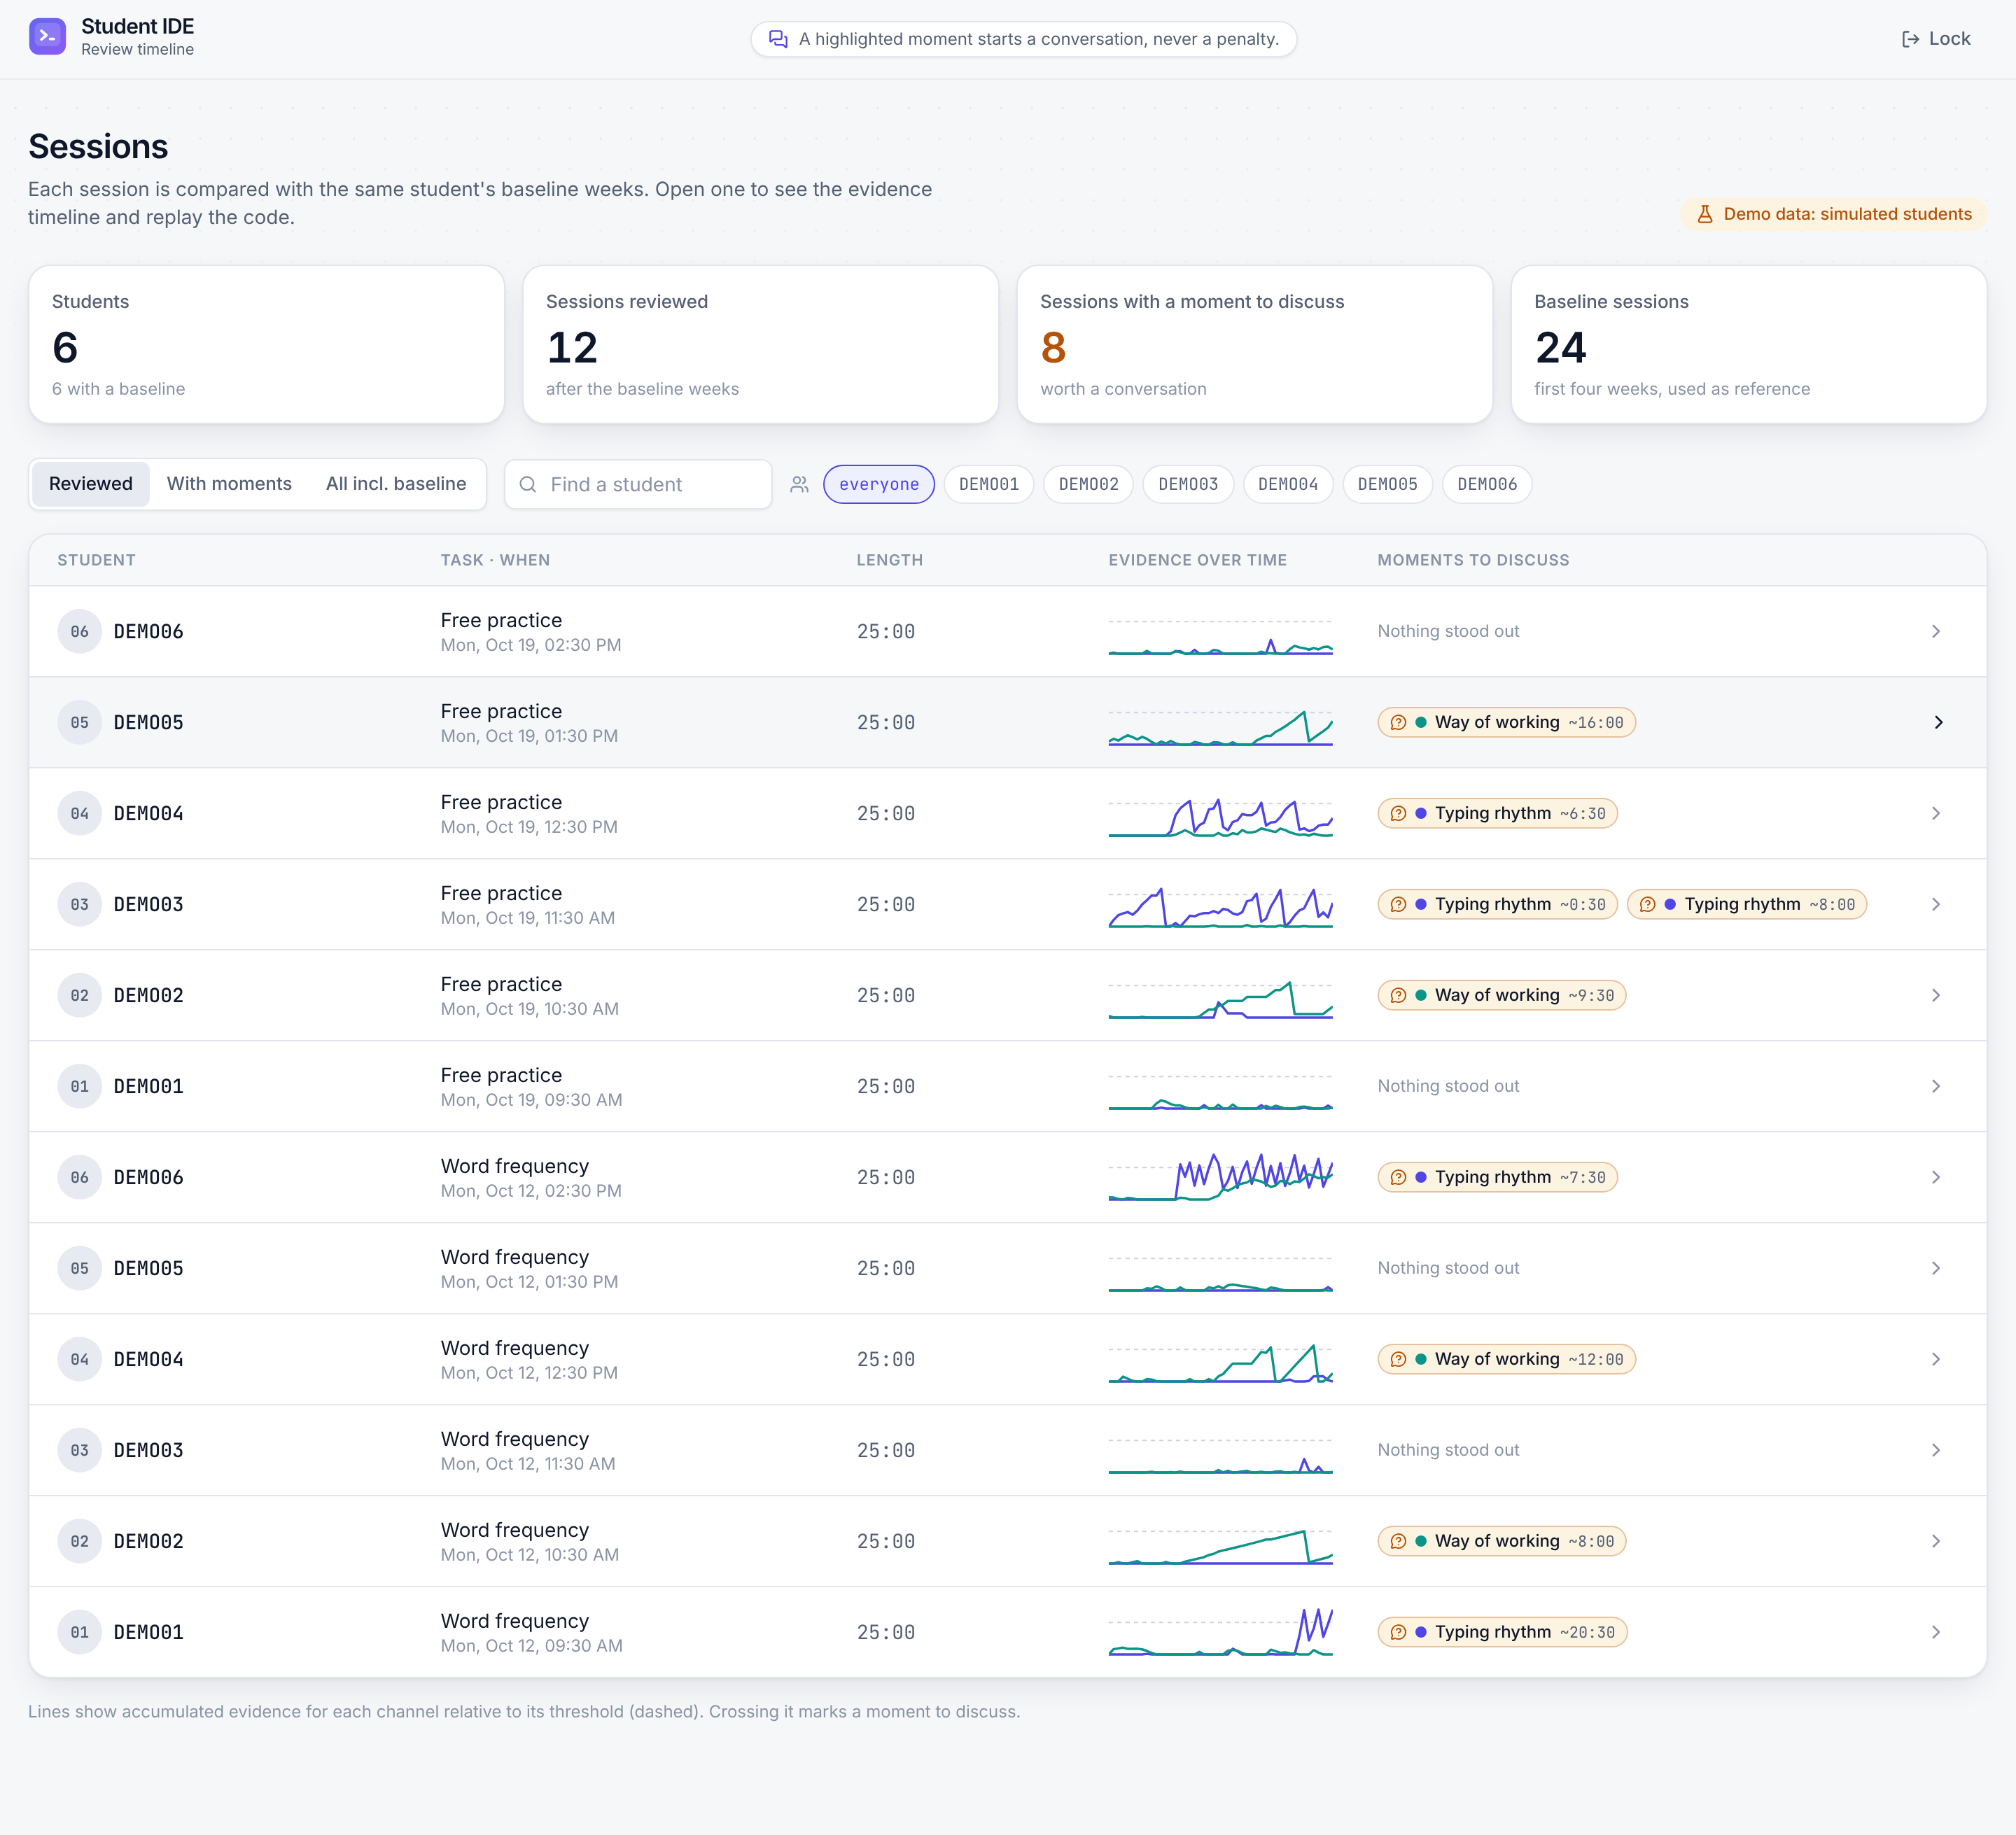
\includegraphics[width=\linewidth]{review/review-light-02-overview}
  \caption{Review overview on simulated students: each row shows every
  channel's accumulated evidence relative to the threshold (dashed) and
  the moments to discuss, with the channel that found them.}
  \label{fig:review-overview}
\end{figure}

\begin{figure}[ht]
  \centering
  \begin{subfigure}{\textwidth}
    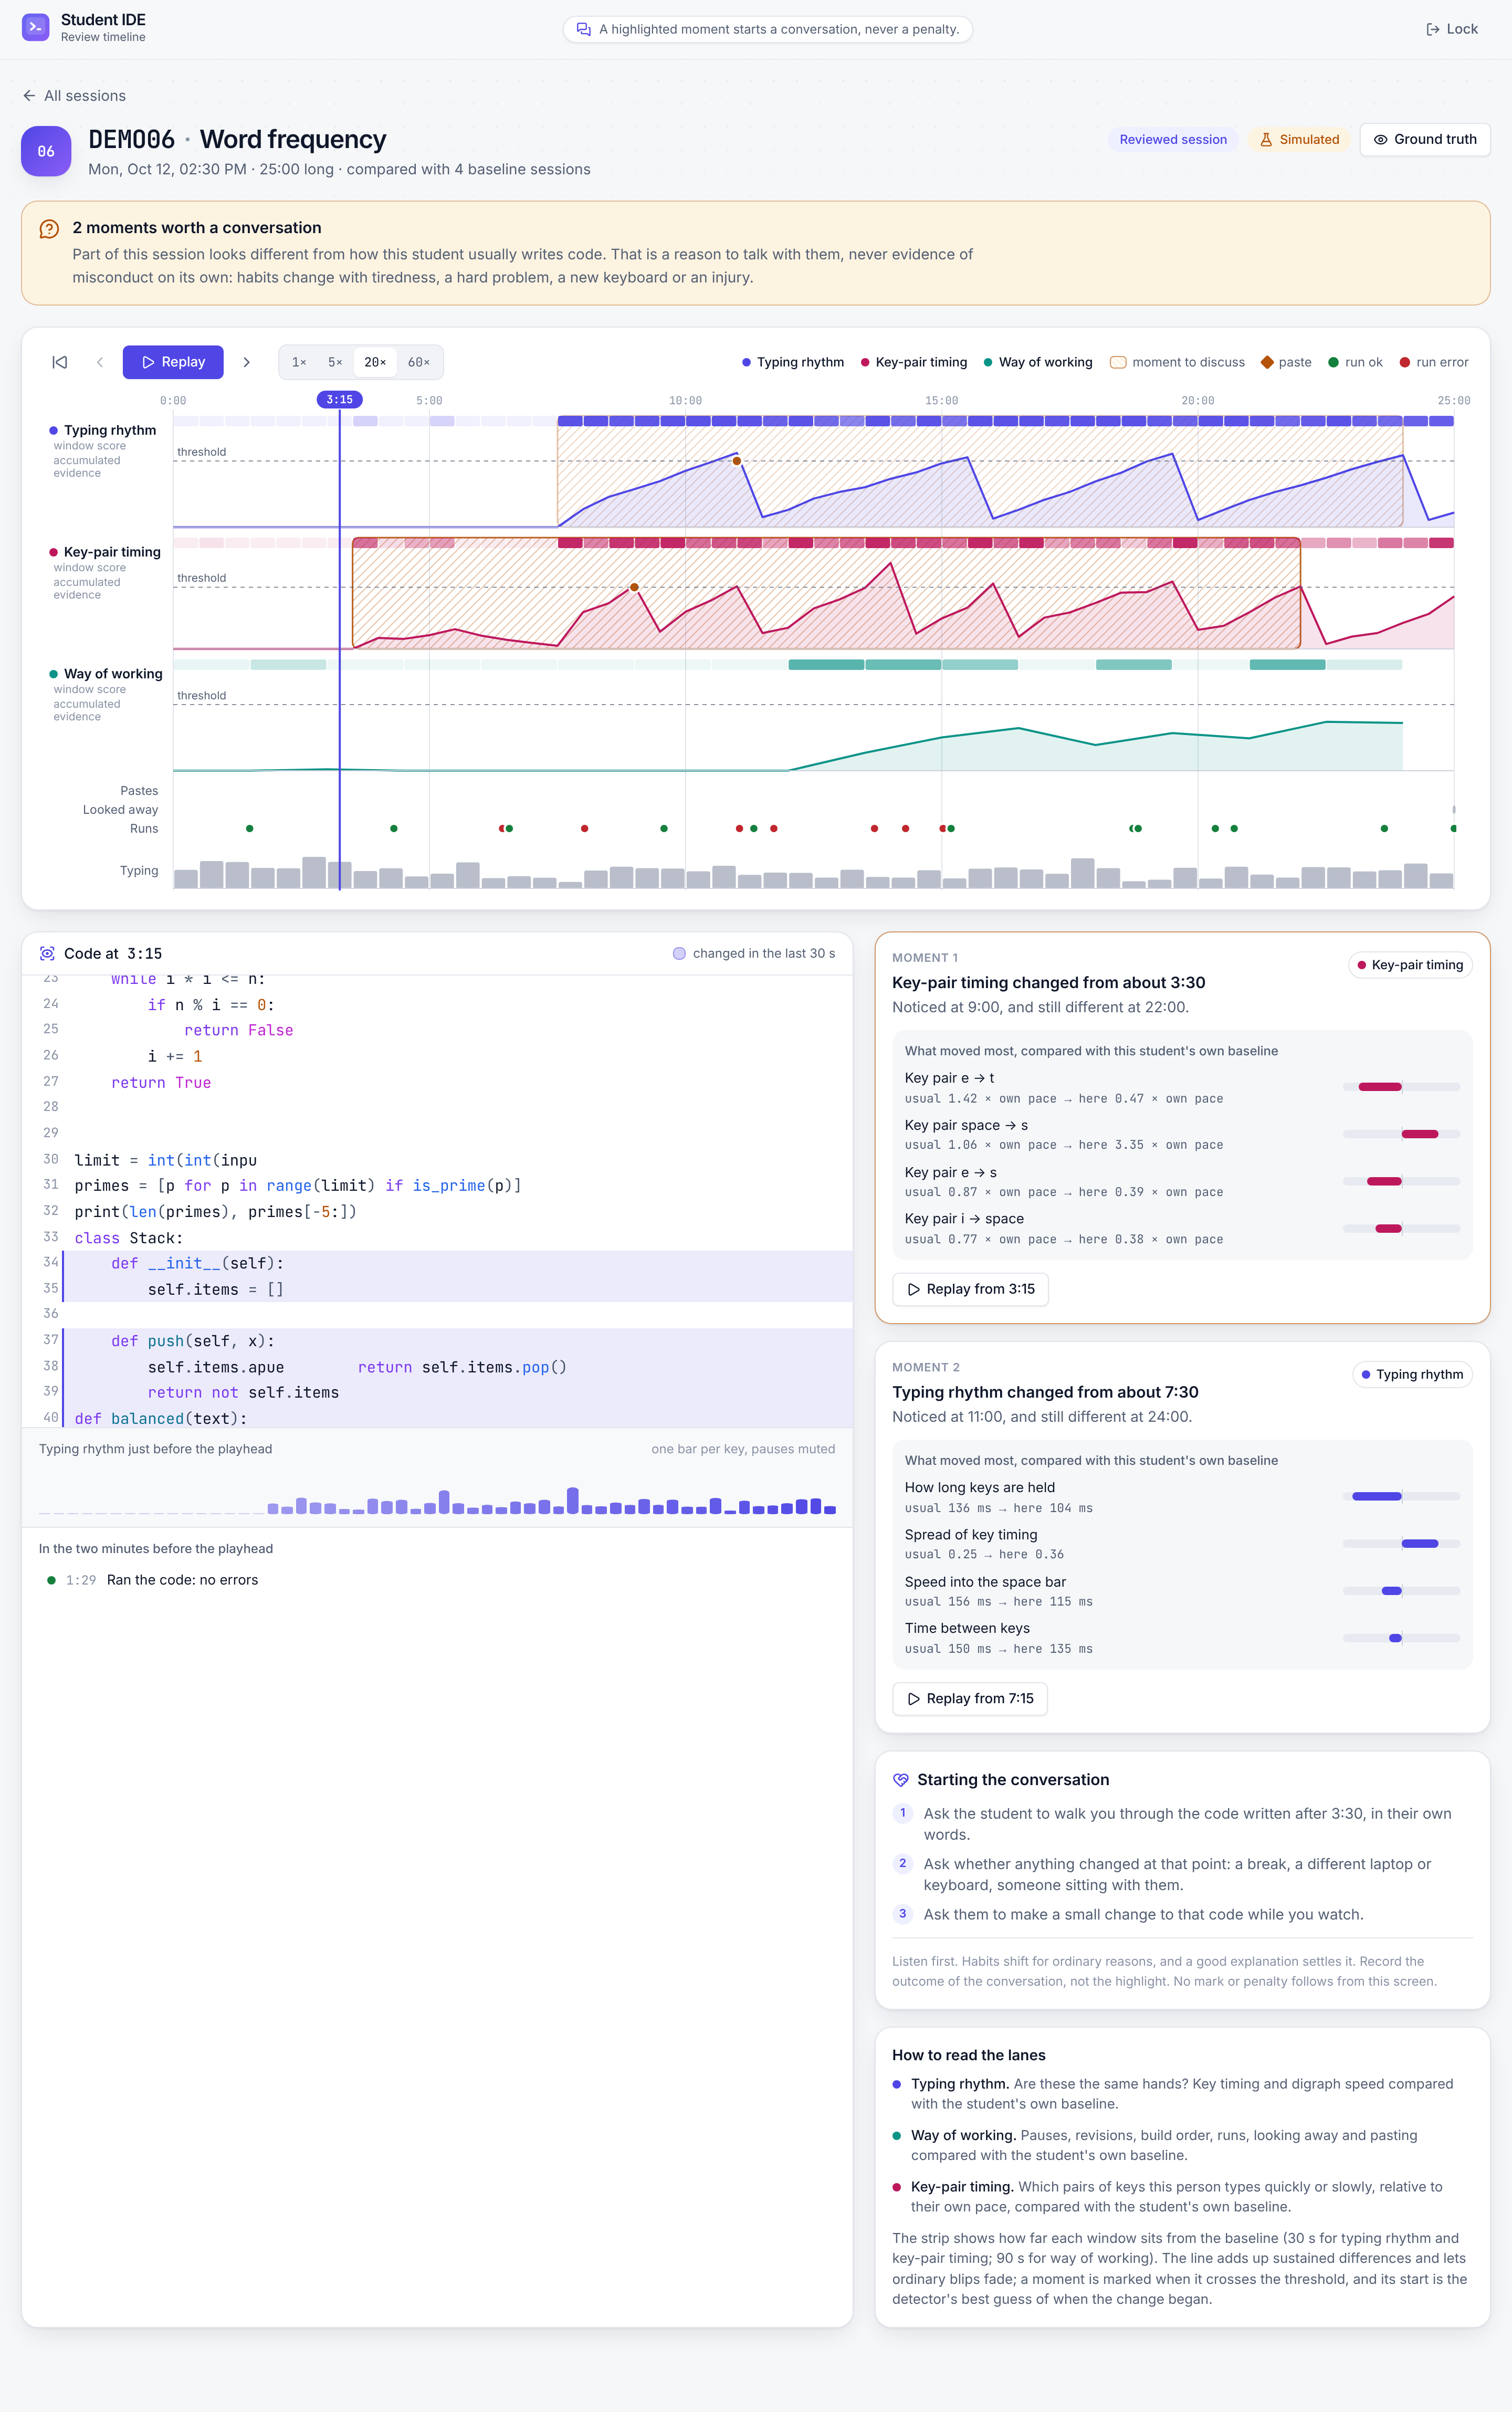
\includegraphics[width=\linewidth]{review/review-light-03-session-takeover}
    \caption{A simulated takeover: the typing-rhythm and key-pair lanes mark
    moments; the replay shows the code at the playhead.}
  \end{subfigure}\\[1ex]
  \begin{subfigure}{\textwidth}
    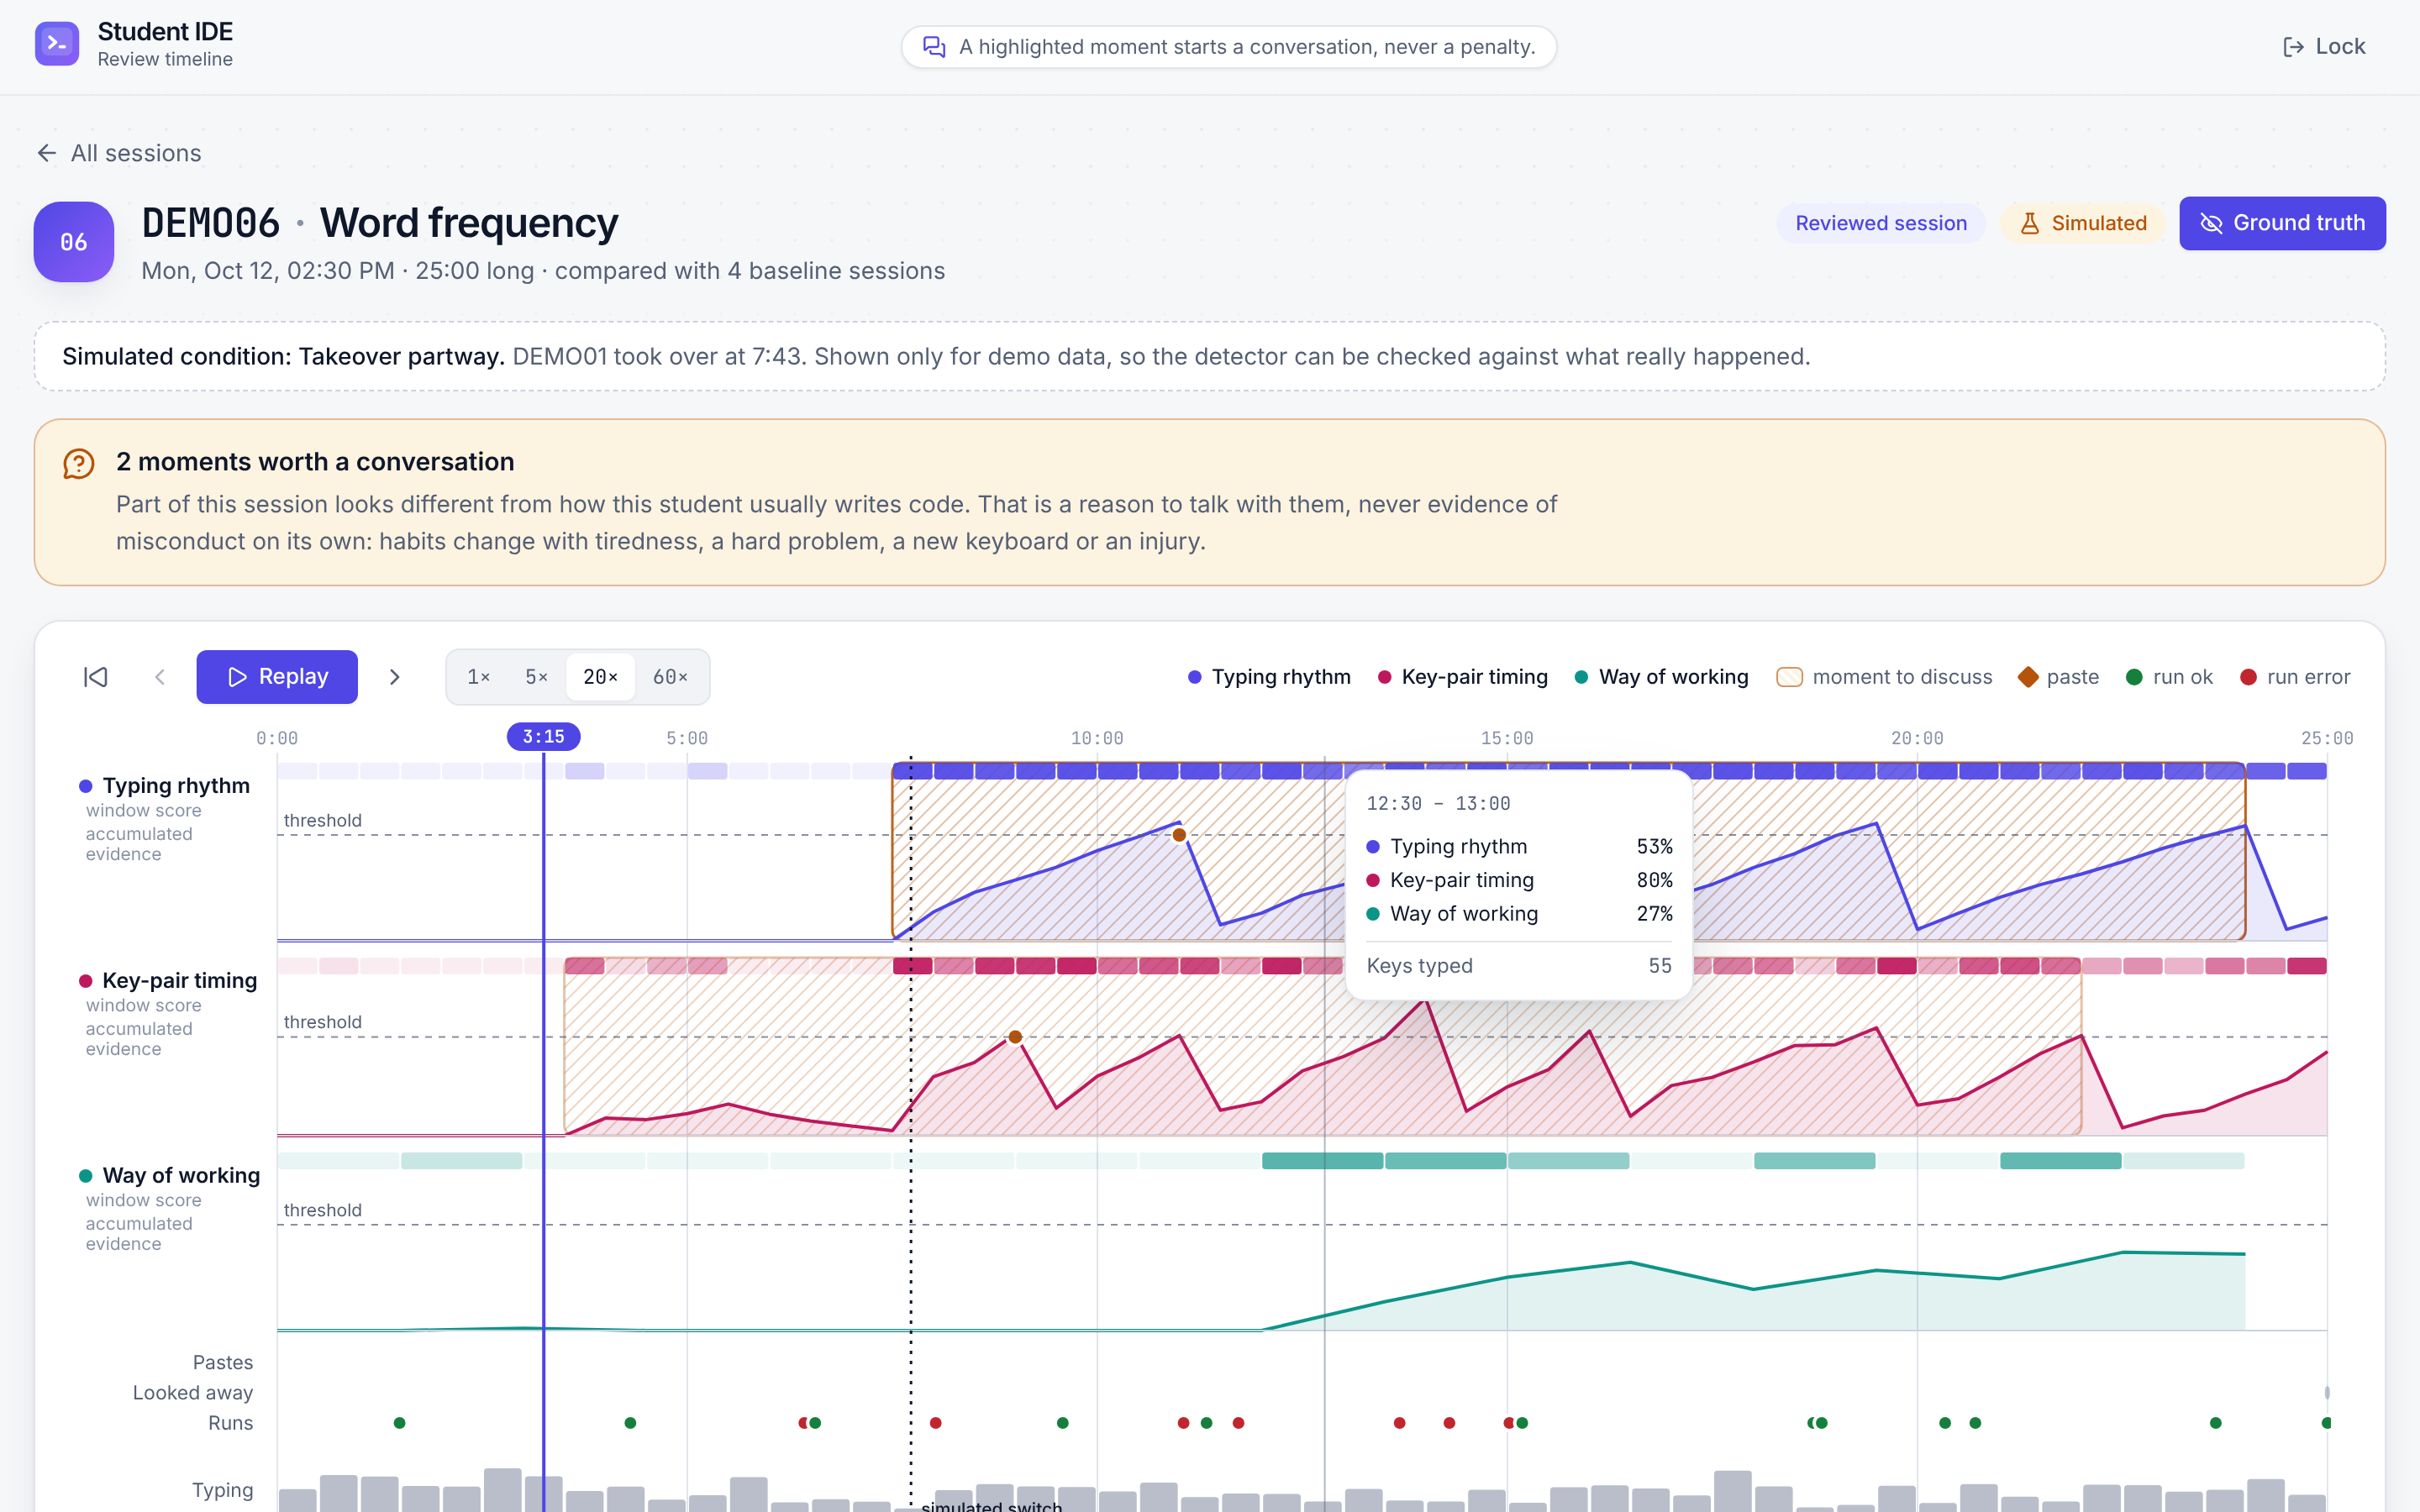
\includegraphics[width=\linewidth]{review/review-light-04-takeover-truth-hover}
    \caption{Same session with the simulated ground truth (switch at 7:43)
    overlaid and the hover read-out for one window. The key-pair lane's
    first moment is dated well before the switch, a reminder that the
    estimated start is a guess.}
  \end{subfigure}
  \caption{Session review timeline. Light and dark versions of every
  screen are in \texttt{snapshots/review/}.}
  \label{fig:review-session}
\end{figure}
